% Options for packages loaded elsewhere
\PassOptionsToPackage{unicode}{hyperref}
\PassOptionsToPackage{hyphens}{url}
%
\documentclass[
]{tufte-pandoc}


% Use upquote if available, for straight quotes in verbatim environments
\IfFileExists{upquote.sty}{\usepackage{upquote}}{}
\IfFileExists{microtype.sty}{% use microtype if available
  \usepackage[]{microtype}
  \UseMicrotypeSet[protrusion]{basicmath} % disable protrusion for tt fonts
}{}
\makeatletter
\@ifundefined{KOMAClassName}{% if non-KOMA class
  \IfFileExists{parskip.sty}{%
    \usepackage{parskip}
  }{% else
    \setlength{\parindent}{0pt}
    \setlength{\parskip}{6pt plus 2pt minus 1pt}}
}{% if KOMA class
  \KOMAoptions{parskip=half}}
\makeatother
\usepackage{xcolor}
\newcommand{\passthrough}[1]{#1}
\usepackage{color}
\usepackage{fancyvrb}
\newcommand{\VerbBar}{|}
\newcommand{\VERB}{\Verb[commandchars=\\\{\}]}
\DefineVerbatimEnvironment{Highlighting}{Verbatim}{commandchars=\\\{\}}
% Add ',fontsize=\small' for more characters per line
\newenvironment{Shaded}{}{}
\newcommand{\AlertTok}[1]{\textcolor[rgb]{1.00,0.00,0.00}{\textbf{#1}}}
\newcommand{\AnnotationTok}[1]{\textcolor[rgb]{0.38,0.63,0.69}{\textbf{\textit{#1}}}}
\newcommand{\AttributeTok}[1]{\textcolor[rgb]{0.49,0.56,0.16}{#1}}
\newcommand{\BaseNTok}[1]{\textcolor[rgb]{0.25,0.63,0.44}{#1}}
\newcommand{\BuiltInTok}[1]{#1}
\newcommand{\CharTok}[1]{\textcolor[rgb]{0.25,0.44,0.63}{#1}}
\newcommand{\CommentTok}[1]{\textcolor[rgb]{0.38,0.63,0.69}{\textit{#1}}}
\newcommand{\CommentVarTok}[1]{\textcolor[rgb]{0.38,0.63,0.69}{\textbf{\textit{#1}}}}
\newcommand{\ConstantTok}[1]{\textcolor[rgb]{0.53,0.00,0.00}{#1}}
\newcommand{\ControlFlowTok}[1]{\textcolor[rgb]{0.00,0.44,0.13}{\textbf{#1}}}
\newcommand{\DataTypeTok}[1]{\textcolor[rgb]{0.56,0.13,0.00}{#1}}
\newcommand{\DecValTok}[1]{\textcolor[rgb]{0.25,0.63,0.44}{#1}}
\newcommand{\DocumentationTok}[1]{\textcolor[rgb]{0.73,0.13,0.13}{\textit{#1}}}
\newcommand{\ErrorTok}[1]{\textcolor[rgb]{1.00,0.00,0.00}{\textbf{#1}}}
\newcommand{\ExtensionTok}[1]{#1}
\newcommand{\FloatTok}[1]{\textcolor[rgb]{0.25,0.63,0.44}{#1}}
\newcommand{\FunctionTok}[1]{\textcolor[rgb]{0.02,0.16,0.49}{#1}}
\newcommand{\ImportTok}[1]{#1}
\newcommand{\InformationTok}[1]{\textcolor[rgb]{0.38,0.63,0.69}{\textbf{\textit{#1}}}}
\newcommand{\KeywordTok}[1]{\textcolor[rgb]{0.00,0.44,0.13}{\textbf{#1}}}
\newcommand{\NormalTok}[1]{#1}
\newcommand{\OperatorTok}[1]{\textcolor[rgb]{0.40,0.40,0.40}{#1}}
\newcommand{\OtherTok}[1]{\textcolor[rgb]{0.00,0.44,0.13}{#1}}
\newcommand{\PreprocessorTok}[1]{\textcolor[rgb]{0.74,0.48,0.00}{#1}}
\newcommand{\RegionMarkerTok}[1]{#1}
\newcommand{\SpecialCharTok}[1]{\textcolor[rgb]{0.25,0.44,0.63}{#1}}
\newcommand{\SpecialStringTok}[1]{\textcolor[rgb]{0.73,0.40,0.53}{#1}}
\newcommand{\StringTok}[1]{\textcolor[rgb]{0.25,0.44,0.63}{#1}}
\newcommand{\VariableTok}[1]{\textcolor[rgb]{0.10,0.09,0.49}{#1}}
\newcommand{\VerbatimStringTok}[1]{\textcolor[rgb]{0.25,0.44,0.63}{#1}}
\newcommand{\WarningTok}[1]{\textcolor[rgb]{0.38,0.63,0.69}{\textbf{\textit{#1}}}}
\usepackage{longtable,booktabs,array}
\usepackage{calc} % for calculating minipage widths
% Correct order of tables after \paragraph or \subparagraph
\usepackage{etoolbox}
\makeatletter
\patchcmd\longtable{\par}{\if@noskipsec\mbox{}\fi\par}{}{}
\makeatother
% Allow footnotes in longtable head/foot
\IfFileExists{footnotehyper.sty}{\usepackage{footnotehyper}}{\usepackage{footnote}}
\makesavenoteenv{longtable}
\usepackage{graphicx}
\makeatletter
\def\maxwidth{\ifdim\Gin@nat@width>\linewidth\linewidth\else\Gin@nat@width\fi}
\def\maxheight{\ifdim\Gin@nat@height>\textheight\textheight\else\Gin@nat@height\fi}
\makeatother
% Scale images if necessary, so that they will not overflow the page
% margins by default, and it is still possible to overwrite the defaults
% using explicit options in \includegraphics[width, height, ...]{}
\setkeys{Gin}{width=\maxwidth,height=\maxheight,keepaspectratio}
% Set default figure placement to htbp
\makeatletter
\def\fps@figure{htbp}
\makeatother
\usepackage[normalem]{ulem}
\setlength{\emergencystretch}{3em} % prevent overfull lines
\providecommand{\tightlist}{%
  \setlength{\itemsep}{0pt}\setlength{\parskip}{0pt}}
\setcounter{secnumdepth}{3}

\IfFileExists{bookmark.sty}{\usepackage{bookmark}}{\usepackage{hyperref}}
\IfFileExists{xurl.sty}{\usepackage{xurl}}{} % add URL line breaks if available
\urlstyle{same} % disable monospaced font for URLs
\hypersetup{
  pdftitle={Test pandoc → tufte-style-article},
  pdfauthor={Sylvain Kern},
  hidelinks,
  pdfcreator={LaTeX via pandoc}}

\title{Test pandoc → tufte-style-article}
\author{Sylvain Kern}
\date{}

\begin{document}
\maketitle


\setcounter{tocdepth}{2}
\tableofcontents

\hypertarget{markdown-kitchen-sink}{%
\section{Markdown Kitchen Sink}\label{markdown-kitchen-sink}}

This file is
https://github.com/adam-p/markdown-here/wiki/Markdown-Cheatsheet plus a
few fixes and additions. Used by
\href{https://github.com/obedm503/bootmark}{obedm503/bootmark} to
\href{https://obedm503.github.io/bootmark/docs/markdown-cheatsheet.html}{demonstrate}
it's styling features.

This is intended as a quick reference and showcase. For more complete
info, see \href{http://daringfireball.net/projects/markdown/}{John
Gruber's original spec} and the
\href{http://github.github.com/github-flavored-markdown/}{Github-flavored
Markdown info page}.

Note that there is also a \href{./Markdown-Here-Cheatsheet}{Cheatsheet
specific to Markdown Here} if that's what you're looking for. You can
also check out \href{./Other-Markdown-Tools}{more Markdown tools}.

\hypertarget{headers}{%
\subsection{Headers}\label{headers}}

\begin{Shaded}
\begin{Highlighting}[]
\NormalTok{\# H1}
\NormalTok{\#\# H2}
\NormalTok{\#\#\# H3}
\NormalTok{\#\#\#\# H4}
\NormalTok{\#\#\#\#\# H5}
\NormalTok{\#\#\#\#\#\# H6}

\NormalTok{Alternatively, for H1 and H2, an underline{-}ish style:}

\NormalTok{Alt{-}H1}
\NormalTok{======}

\NormalTok{Alt{-}H2}
\NormalTok{{-}{-}{-}{-}{-}{-}}
\end{Highlighting}
\end{Shaded}

\hypertarget{h1}{%
\section{H1}\label{h1}}

\hypertarget{h2}{%
\subsection{H2}\label{h2}}

\hypertarget{h3}{%
\subsubsection{H3}\label{h3}}

\hypertarget{h4}{%
\paragraph{H4}\label{h4}}

\hypertarget{h5}{%
\subparagraph{H5}\label{h5}}

H6

Alternatively, for H1 and H2, an underline-ish style:

\hypertarget{alt-h1}{%
\section{Alt-H1}\label{alt-h1}}

\hypertarget{alt-h2}{%
\subsection{Alt-H2}\label{alt-h2}}

\hypertarget{emphasis}{%
\subsection{Emphasis}\label{emphasis}}

\begin{Shaded}
\begin{Highlighting}[]
\NormalTok{Emphasis, aka italics, with *asterisks* or \_underscores\_.}

\NormalTok{Strong emphasis, aka bold, with **asterisks** or \_\_underscores\_\_.}

\NormalTok{Combined emphasis with **asterisks and \_underscores\_**.}

\NormalTok{Strikethrough uses two tildes. \textasciitilde{}\textasciitilde{}Scratch this.\textasciitilde{}\textasciitilde{}}
\end{Highlighting}
\end{Shaded}

Emphasis, aka italics, with \emph{asterisks} or \emph{underscores}.

Strong emphasis, aka bold, with \textbf{asterisks} or
\textbf{underscores}.

Combined emphasis with \textbf{asterisks and \emph{underscores}}.

Strikethrough uses two tildes. \sout{Scratch this.}

\hypertarget{lists}{%
\subsection{Lists}\label{lists}}

(In this example, leading and trailing spaces are shown with with dots:
)

\begin{Shaded}
\begin{Highlighting}[]
\NormalTok{1. First ordered list item}
\NormalTok{2. Another item}
\NormalTok{  * Unordered sub{-}list.}
\NormalTok{1. Actual numbers don\textquotesingle{}t matter, just that it\textquotesingle{}s a number}
\NormalTok{  1. Ordered sub{-}list}
\NormalTok{4. And another item.}

\NormalTok{   You can have properly indented paragraphs within list items. Notice the blank line above, and the leading spaces (at least one, but we\textquotesingle{}ll use three here to also align the raw Markdown).}

\NormalTok{   To have a line break without a paragraph, you will need to use two trailing spaces.}
\NormalTok{   Note that this line is separate, but within the same paragraph.}
\NormalTok{   (This is contrary to the typical GFM line break behaviour, where trailing spaces are not required.)}

\NormalTok{* Unordered list can use asterisks}
\NormalTok{{-} Or minuses}
\NormalTok{+ Or pluses}
\end{Highlighting}
\end{Shaded}

\begin{enumerate}
\def\labelenumi{\arabic{enumi}.}
\tightlist
\item
  First ordered list item
\item
  Another item
\end{enumerate}

\begin{itemize}
\tightlist
\item
  Unordered sub-list.
\end{itemize}

\begin{enumerate}
\def\labelenumi{\arabic{enumi}.}
\item
  Actual numbers don't matter, just that it's a number
\item
  Ordered sub-list
\item
  And another item.

  You can have properly indented paragraphs within list items. Notice
  the blank line above, and the leading spaces (at least one, but we'll
  use three here to also align the raw Markdown).

  To have a line break without a paragraph, you will need to use two
  trailing spaces. Note that this line is separate, but within the same
  paragraph. (This is contrary to the typical GFM line break behaviour,
  where trailing spaces are not required.)
\end{enumerate}

\begin{itemize}
\tightlist
\item
  Unordered list can use asterisks
\item
  Or minuses
\item
  Or pluses
\end{itemize}

\hypertarget{links}{%
\subsection{Links}\label{links}}

There are two ways to create links.

\begin{Shaded}
\begin{Highlighting}[]
\NormalTok{[I\textquotesingle{}m an inline{-}style link](https://www.google.com)}

\NormalTok{[I\textquotesingle{}m an inline{-}style link with title](https://www.google.com "Google\textquotesingle{}s Homepage")}

\NormalTok{[I\textquotesingle{}m a reference{-}style link][Arbitrary case{-}insensitive reference text]}

\NormalTok{[I\textquotesingle{}m a relative reference to a repository file](../blob/master/LICENSE)}

\NormalTok{[You can use numbers for reference{-}style link definitions][1]}

\NormalTok{Or leave it empty and use the [link text itself].}

\NormalTok{URLs and URLs in angle brackets will automatically get turned into links.}
\NormalTok{http://www.example.com or \textless{}http://www.example.com\textgreater{} and sometimes}
\NormalTok{example.com (but not on Github, for example).}

\NormalTok{Some text to show that the reference links can follow later.}

\NormalTok{[arbitrary case{-}insensitive reference text]: https://www.mozilla.org}
\NormalTok{[1]: http://slashdot.org}
\NormalTok{[link text itself]: http://www.reddit.com}
\end{Highlighting}
\end{Shaded}

\href{https://www.google.com}{I'm an inline-style link}

\href{https://www.google.com}{I'm an inline-style link with title}

\href{https://www.mozilla.org}{I'm a reference-style link}

\href{../blob/master/LICENSE}{I'm a relative reference to a repository
file}

\href{http://slashdot.org}{You can use numbers for reference-style link
definitions}

Or leave it empty and use the \href{http://www.reddit.com}{link text
itself}.

URLs and URLs in angle brackets will automatically get turned into
links. http://www.example.com or \url{http://www.example.com} and
sometimes example.com (but not on Github, for example).

Some text to show that the reference links can follow later.

\hypertarget{images}{%
\subsection{Images}\label{images}}

\begin{Shaded}
\begin{Highlighting}[]
\NormalTok{Here\textquotesingle{}s our logo (hover to see the title text):}

\NormalTok{Inline{-}style:}
\NormalTok{![alt text](https://github.com/adam{-}p/markdown{-}here/raw/master/src/common/images/icon48.png "Logo Title Text 1")}

\NormalTok{Reference{-}style:}
\NormalTok{![alt text][logo]}

\NormalTok{[logo]: https://github.com/adam{-}p/markdown{-}here/raw/master/src/common/images/icon48.png "Logo Title Text 2"}
\end{Highlighting}
\end{Shaded}

Here's our logo (hover to see the title text):

\hypertarget{code-and-syntax-highlighting}{%
\subsection{Code and Syntax
Highlighting}\label{code-and-syntax-highlighting}}

Code blocks are part of the Markdown spec, but syntax highlighting
isn't. However, many renderers -- like Github's and \emph{Markdown Here}
-- support syntax highlighting. Which languages are supported and how
those language names should be written will vary from renderer to
renderer. \emph{Markdown Here} supports highlighting for dozens of
languages (and not-really-languages, like diffs and HTTP headers); to
see the complete list, and how to write the language names, see the
\href{http://softwaremaniacs.org/media/soft/highlight/test.html}{highlight.js
demo page}.

\begin{Shaded}
\begin{Highlighting}[]
\NormalTok{Inline \textasciigrave{}code\textasciigrave{} has \textasciigrave{}back{-}ticks around\textasciigrave{} it.}
\end{Highlighting}
\end{Shaded}

Inline \texttt{code} has \texttt{back-ticks\ around} it.

Blocks of code are either fenced by lines with three back-ticks ```, or
are indented with four spaces. I recommend only using the fenced code
blocks -- they're easier and only they support syntax highlighting.

\begin{Shaded}
\begin{Highlighting}[]
\KeywordTok{var}\NormalTok{ s }\OperatorTok{=} \StringTok{"JavaScript syntax highlighting"}\OperatorTok{;}
\FunctionTok{alert}\NormalTok{(s)}\OperatorTok{;}
\end{Highlighting}
\end{Shaded}

\begin{Shaded}
\begin{Highlighting}[]
\NormalTok{s }\OperatorTok{=} \StringTok{"Python syntax highlighting"}
\BuiltInTok{print}\NormalTok{ s}
\end{Highlighting}
\end{Shaded}

\begin{verbatim}
No language indicated, so no syntax highlighting in Markdown Here (varies on Github).
But let's throw in a <b>tag</b>.
\end{verbatim}

\hypertarget{tables}{%
\subsection{Tables}\label{tables}}

Tables aren't part of the core Markdown spec, but they are part of GFM
and \emph{Markdown Here} supports them. They are an easy way of adding
tables to your email -- a task that would otherwise require copy-pasting
from another application.

\begin{Shaded}
\begin{Highlighting}[]
\NormalTok{Colons can be used to align columns.}

\NormalTok{| Tables        | Are           | Cool  |}
\NormalTok{| {-}{-}{-}{-}{-}{-}{-}{-}{-}{-}{-}{-}{-} |:{-}{-}{-}{-}{-}{-}{-}{-}{-}{-}{-}{-}{-}:| {-}{-}{-}{-}{-}:|}
\NormalTok{| col 3 is      | right{-}aligned | $1600 |}
\NormalTok{| col 2 is      | centered      |   $12 |}
\NormalTok{| zebra stripes | are neat      |    $1 |}

\NormalTok{There must be at least 3 dashes separating each header cell.}
\NormalTok{The outer pipes (|) are optional, and you don\textquotesingle{}t need to make the}
\NormalTok{raw Markdown line up prettily. You can also use inline Markdown.}

\NormalTok{Markdown | Less | Pretty}
\NormalTok{{-}{-}{-} | {-}{-}{-} | {-}{-}{-}}
\NormalTok{*Still* | \textasciigrave{}renders\textasciigrave{} | **nicely**}
\NormalTok{1 | 2 | 3}
\end{Highlighting}
\end{Shaded}

Colons can be used to align columns.

\begin{longtable}[]{@{}lcr@{}}
\toprule()
Tables & Are & Cool \\
\midrule()
\endhead
col 3 is & right-aligned & \$1600 \\
col 2 is & centered & \$12 \\
zebra stripes & are neat & \$1 \\
\bottomrule()
\end{longtable}

There must be at least 3 dashes separating each header cell. The outer
pipes (\textbar) are optional, and you don't need to make the raw
Markdown line up prettily. You can also use inline Markdown.

\begin{longtable}[]{@{}lll@{}}
\toprule()
Markdown & Less & Pretty \\
\midrule()
\endhead
\emph{Still} & \texttt{renders} & \textbf{nicely} \\
1 & 2 & 3 \\
\bottomrule()
\end{longtable}

\hypertarget{blockquotes}{%
\subsection{Blockquotes}\label{blockquotes}}

\begin{Shaded}
\begin{Highlighting}[]
\NormalTok{\textgreater{} Blockquotes are very handy in email to emulate reply text.}
\NormalTok{\textgreater{} This line is part of the same quote.}

\NormalTok{Quote break.}

\NormalTok{\textgreater{} This is a very long line that will still be quoted properly when it wraps. Oh boy let\textquotesingle{}s keep writing to make sure this is long enough to actually wrap for everyone. Oh, you can *put* **Markdown** into a blockquote.}
\end{Highlighting}
\end{Shaded}

\begin{quote}
Blockquotes are very handy in email to emulate reply text. This line is
part of the same quote.
\end{quote}

Quote break.

\begin{quote}
This is a very long line that will still be quoted properly when it
wraps. Oh boy let's keep writing to make sure this is long enough to
actually wrap for everyone. Oh, you can \emph{put} \textbf{Markdown}
into a blockquote.
\end{quote}

\hypertarget{inline-html}{%
\subsection{Inline HTML}\label{inline-html}}

You can also use raw HTML in your Markdown, and it'll mostly work pretty
well.

\begin{Shaded}
\begin{Highlighting}[]
\NormalTok{\textless{}dl\textgreater{}}
\NormalTok{  \textless{}dt\textgreater{}Definition list\textless{}/dt\textgreater{}}
\NormalTok{  \textless{}dd\textgreater{}Is something people use sometimes.\textless{}/dd\textgreater{}}

\NormalTok{  \textless{}dt\textgreater{}Markdown in HTML\textless{}/dt\textgreater{}}
\NormalTok{  \textless{}dd\textgreater{}Does *not* work **very** well. Use HTML \textless{}em\textgreater{}tags\textless{}/em\textgreater{}.\textless{}/dd\textgreater{}}
\NormalTok{\textless{}/dl\textgreater{}}
\end{Highlighting}
\end{Shaded}

Definition list

Is something people use sometimes.

Markdown in HTML

Does \emph{not} work \textbf{very} well. Use HTML tags.

\hypertarget{horizontal-rule}{%
\subsection{Horizontal Rule}\label{horizontal-rule}}

\begin{verbatim}
Three or more...

---

Hyphens

***

Asterisks

___

Underscores
\end{verbatim}

Three or more\ldots{}

\begin{center}\rule{0.5\linewidth}{0.5pt}\end{center}

Hyphens

\begin{center}\rule{0.5\linewidth}{0.5pt}\end{center}

Asterisks

\begin{center}\rule{0.5\linewidth}{0.5pt}\end{center}

Underscores

\hypertarget{line-breaks}{%
\subsection{Line Breaks}\label{line-breaks}}

My basic recommendation for learning how line breaks work is to
experiment and discover -- hit \textless Enter\textgreater{} once (i.e.,
insert one newline), then hit it twice (i.e., insert two newlines), see
what happens. You'll soon learn to get what you want. ``Markdown
Toggle'' is your friend.

Here are some things to try out:

\begin{verbatim}
Here's a line for us to start with.

This line is separated from the one above by two newlines, so it will be a *separate paragraph*.

This line is also a separate paragraph, but...
This line is only separated by a single newline, so it's a separate line in the *same paragraph*.
\end{verbatim}

Here's a line for us to start with.

This line is separated from the one above by two newlines, so it will be
a \emph{separate paragraph}.

This line is also begins a separate paragraph, but\ldots{} This line is
only separated by a single newline, so it's a separate line in the
\emph{same paragraph}.

(Technical note: \emph{Markdown Here} uses GFM line breaks, so there's
no need to use MD's two-space line breaks.)

\hypertarget{youtube-videos}{%
\subsection{YouTube Videos}\label{youtube-videos}}

They can't be added directly but you can add an image with a link to the
video like this:

\begin{Shaded}
\begin{Highlighting}[]
\NormalTok{\textless{}a href="http://www.youtube.com/watch?feature=player\_embedded\&v=YOUTUBE\_VIDEO\_ID\_HERE}
\NormalTok{" target="\_blank"\textgreater{}\textless{}img src="http://img.youtube.com/vi/YOUTUBE\_VIDEO\_ID\_HERE/0.jpg"}
\NormalTok{alt="IMAGE ALT TEXT HERE" width="240" height="180" border="10" /\textgreater{}\textless{}/a\textgreater{}}
\end{Highlighting}
\end{Shaded}

Or, in pure Markdown, but losing the image sizing and border:

\begin{Shaded}
\begin{Highlighting}[]
\NormalTok{[![IMAGE ALT TEXT HERE](http://img.youtube.com/vi/YOUTUBE\_VIDEO\_ID\_HERE/0.jpg)](http://www.youtube.com/watch?v=YOUTUBE\_VIDEO\_ID\_HERE)}
\end{Highlighting}
\end{Shaded}

\hypertarget{abstract}{%
\section*{Abstract}\label{abstract}}
\addcontentsline{toc}{section}{Abstract}

At vero eos et accusamus et iusto odio dignissimos ducimus qui
blanditiis praesentium voluptatum deleniti atque corrupti quos dolores
et quas molestias excepturi sint occaecati cupiditate non provident,
similique sunt in culpa qui officia deserunt mollitia animi, id est
laborum et dolorum fuga. Et harum quidem rerum facZilis est et expedita
distinctio. Nam libero tempore, cum soluta nobis est eligendi optio
cumque nihil impedit quo minus id quod maxime placeat facere possimus,
omnis voluptas assumenda est, omnis dolor repellendus. Temporibus autem
quibusdam et aut officiis debitis aut rerum necessitatibus saepe eveniet
ut et voluptates repudiandae sint et molestiae non recusandae. Itaque
earum rerum hic tenetur a sapiente delectus, ut aut reiciendis
voluptatibus maiores alias consequatur aut perferendis doloribus
asperiores repellat.

\hypertarget{acknowledgements}{%
\section*{Acknowledgements}\label{acknowledgements}}
\addcontentsline{toc}{section}{Acknowledgements}

My man

The family

The hood

\hypertarget{h1-chapter-title}{%
\section{H1: chapter title}\label{h1-chapter-title}}

\hypertarget{header}{%
\subsubsection*{header}\label{header}}
\addcontentsline{toc}{subsubsection}{header}

\hypertarget{all-headings-this-is-level-two}{%
\subsection{All headings (this is level
two)}\label{all-headings-this-is-level-two}}

\hypertarget{level-three}{%
\subsubsection{Level three}\label{level-three}}

\hypertarget{level-four}{%
\paragraph{Level four}\label{level-four}}

\hypertarget{level-five-unnumbered}{%
\subparagraph*{Level five (unnumbered)}\label{level-five-unnumbered}}
\addcontentsline{toc}{subparagraph}{Level five (unnumbered)}

Level six

\hypertarget{harmony-counterpoint-paragraph-flow-balance}{%
\subsection{Harmony \& counterpoint (paragraph flow \&
balance)}\label{harmony-counterpoint-paragraph-flow-balance}}

Lorem ipsum dolor sit amet, consectetur adipiscing elit, sed do eiusmod
tempor incididunt ut labore et dolore magna aliqua. Eget lorem dolor sed
viverra ipsum nunc aliquet bibendum enim. Felis imperdiet proin
fermentum leo vel orci porta non pulvinar. Phasellus egestas tellus
rutrum tellus pellentesque eu tincidunt tortor. Congue eu consequat ac
felis donec et odio pellentesque diam. Sit amet nulla facilisi morbi
tempus iaculis urna id. Eget dolor morbi non arcu risus. Nulla facilisi
etiam dignissim diam quis enim lobortis. Mattis ullamcorper velit sed
ullamcorper. Diam volutpat commodo sed egestas egestas fringilla
phasellus. Non nisi est sit amet facilisis.

Aliquet nibh praesent tristique magna sit. Ullamcorper a lacus
vestibulum sed arcu non. Sed risus pretium quam vulputate. In aliquam
sem fringilla ut. Volutpat blandit aliquam etiam erat velit scelerisque
in dictum non. Nec ultrices dui sapien eget mi. Massa placerat duis
ultricies lacus sed turpis. Nulla facilisi etiam dignissim diam quis
enim lobortis scelerisque. Tempus iaculis urna id volutpat lacus. Nulla
facilisi cras fermentum odio eu.

Dignissim diam quis enim lobortis scelerisque fermentum dui faucibus.
Diam quam nulla porttitor massa id. Ultrices mi tempus imperdiet nulla
malesuada pellentesque. Quam lacus suspendisse faucibus interdum posuere
lorem ipsum. Lorem dolor sed viverra ipsum nunc aliquet bibendum enim
facilisis. Blandit cursus risus at ultrices mi. Justo laoreet sit amet
cursus sit amet. Senectus et netus et malesuada fames ac. Faucibus
scelerisque eleifend donec pretium vulputate. Rutrum quisque non tellus
orci ac auctor augue. Mi tempus imperdiet nulla malesuada pellentesque
elit eget gravida. Praesent tristique magna sit amet purus gravida quis
blandit.

Amet purus gravida quis blandit. Tincidunt dui ut ornare lectus sit
amet. Duis ultricies lacus sed turpis tincidunt id aliquet risus
feugiat. Tortor vitae purus faucibus ornare suspendisse sed nisi lacus
sed. Fringilla ut morbi tincidunt augue interdum. Id diam maecenas
ultricies mi eget mauris pharetra et. Pellentesque nec nam aliquam sem
et. Eleifend mi in nulla posuere. Et netus et malesuada fames ac turpis
egestas. Platea dictumst vestibulum rhoncus est pellentesque elit
ullamcorper. Quis risus sed vulputate odio ut.

Urna neque viverra justo nec ultrices. Pulvinar proin gravida hendrerit
lectus a. Velit ut tortor pretium viverra suspendisse potenti nullam.
Eget gravida cum sociis natoque penatibus et. Aliquet sagittis id
consectetur purus ut. Sagittis eu volutpat odio facilisis mauris. Eget
dolor morbi non arcu. Eget velit aliquet sagittis id consectetur purus
ut faucibus. Urna porttitor rhoncus dolor purus non enim praesent
elementum. Senectus et netus et malesuada fames ac turpis egestas.

Tempus iaculis urna id volutpat lacus laoreet. Senectus et netus et
malesuada fames ac turpis egestas maecenas. Nisi est sit amet facilisis
magna etiam tempor orci eu. Nibh praesent tristique magna sit amet. Eget
egestas purus viverra accumsan in nisl. Ullamcorper eget nulla facilisi
etiam dignissim diam quis. Ipsum suspendisse ultrices gravida dictum.
Pellentesque dignissim enim sit amet venenatis urna cursus eget. Nec
tincidunt praesent semper feugiat. Elementum nisi quis eleifend quam
adipiscing. Sed risus pretium quam vulputate dignissim suspendisse in
est ante. Massa ultricies mi quis hendrerit dolor magna eget est lorem.
Condimentum lacinia quis vel eros donec ac odio tempor orci. Sagittis
purus sit amet volutpat consequat mauris. Interdum consectetur libero id
faucibus nisl tincidunt eget. Feugiat nibh sed pulvinar proin gravida
hendrerit. Congue eu consequat ac felis donec et odio. Bibendum arcu
vitae elementum curabitur vitae. Elit scelerisque mauris pellentesque
pulvinar pellentesque habitant morbi tristique.

Eleifend donec pretium vulputate sapien nec. Nunc sed id semper risus in
hendrerit gravida. A diam maecenas sed enim ut. Tempor orci dapibus
ultrices in iaculis nunc sed augue. At consectetur lorem donec massa
sapien faucibus et molestie ac. Natoque penatibus et magnis dis
parturient montes. Tellus in hac habitasse platea dictumst vestibulum
rhoncus. Risus viverra adipiscing at in tellus. Dignissim sodales ut eu
sem integer vitae justo eget. Metus aliquam eleifend mi in nulla
posuere. Turpis nunc eget lorem dolor sed viverra ipsum. Sed velit
dignissim sodales ut eu sem. Vitae purus faucibus ornare suspendisse sed
nisi. Id ornare arcu odio ut sem. Ut venenatis tellus in metus vulputate
eu scelerisque felis. Cursus metus aliquam eleifend mi in. Donec
adipiscing tristique risus nec feugiat. Nibh nisl condimentum id
venenatis a condimentum vitae sapien pellentesque.

Cras fermentum odio eu feugiat pretium. Sed id semper risus in hendrerit
gravida. Dolor sed viverra ipsum nunc. Non blandit massa enim nec dui
nunc mattis. Nunc consequat interdum varius sit amet mattis. Vulputate
dignissim suspendisse in est ante in nibh. Habitant morbi tristique
senectus et netus et malesuada. Venenatis lectus magna fringilla urna
porttitor rhoncus. Lobortis elementum nibh tellus molestie nunc non
blandit massa enim. Volutpat lacus laoreet non curabitur gravida arcu
ac. Amet consectetur adipiscing elit pellentesque habitant. Sed tempus
urna et pharetra pharetra. Quam pellentesque nec nam aliquam. Id velit
ut tortor pretium viverra suspendisse potenti nullam ac.

\hypertarget{line-length-test}{%
\subsubsection{Line length test}\label{line-length-test}}

azertyuiopqsdfghjklmwxcvbnazertyuiopqsdfghjklmwxcvbnazertyuiopqsdfghjklmwxcvbnazertyuiopqsdfghjklmwxcvbn

\hypertarget{unnumbered-section}{%
\subsection*{Unnumbered section}\label{unnumbered-section}}
\addcontentsline{toc}{subsection}{Unnumbered section}

Eleifend donec pretium vulputate sapien nec. Nunc sed id semper risus in
hendrerit gravida. A diam maecenas sed enim ut. Tempor orci dapibus
ultrices in iaculis nunc sed augue. At consectetur lorem donec massa
sapien faucibus et molestie ac. Natoque penatibus et magnis dis
parturient montes. Tellus in hac habitasse platea dictumst vestibulum
rhoncus. Risus viverra adipiscing at in tellus. Dignissim sodales ut eu
sem integer vitae justo eget. Metus aliquam eleifend mi in nulla
posuere. Turpis nunc eget lorem dolor sed viverra ipsum. Sed velit
dignissim sodales ut eu sem. Vitae purus faucibus ornare suspendisse sed
nisi. Id ornare arcu odio ut sem. Ut venenatis tellus in metus vulputate
eu scelerisque felis. Cursus metus aliquam eleifend mi in. Donec
adipiscing tristique risus nec feugiat. Nibh nisl condimentum id
venenatis a condimentum vitae sapien pellentesque.

Cras fermentum odio eu feugiat pretium. Sed id semper risus in hendrerit
gravida. Dolor sed viverra ipsum nunc. Non blandit massa enim nec dui
nunc mattis. Nunc consequat interdum varius sit amet mattis. Vulputate
dignissim suspendisse in est ante in nibh. Habitant morbi tristique
senectus et netus et malesuada. Venenatis lectus magna fringilla urna
porttitor rhoncus. Lobortis elementum nibh tellus molestie nunc non
blandit massa enim. Volutpat lacus laoreet non curabitur gravida arcu
ac. Amet consectetur adipiscing elit pellentesque habitant. Sed tempus
urna et pharetra pharetra. Quam pellentesque nec nam aliquam. Id velit
ut tortor pretium viverra suspendisse potenti nullam ac.

\hypertarget{markdown-features}{%
\subsection{Markdown features}\label{markdown-features}}

Lorem markdownum Niobe, in quae peracta, matrem ubi vates, blanditiis?
\textbf{Dabitur omnia aper} cacumina sensisse in idque passim datum,
lupis terrent Aurora Maia.

\begin{Shaded}
\begin{Highlighting}[]
\FunctionTok{association\_ascii\_domain}\OperatorTok{(}\NormalTok{hoverHibernateMatrix}\OperatorTok{);}
\FunctionTok{left\_memory}\OperatorTok{(}\NormalTok{design}\OperatorTok{,}\NormalTok{ ideReciprocalAtm}\OperatorTok{);}
\DataTypeTok{var}\NormalTok{ kilohertzHost }\OperatorTok{=}\NormalTok{ type\_requirements\_slashdot}\OperatorTok{;}
\end{Highlighting}
\end{Shaded}

Aestus virgo cur languore \textbf{laudamus doluisse} tempora canis,
ausorum habent ab quoque dextra. Cum fecissem excussit patriosque
quodque, et etiam subtemen \textbf{quoque}, papyriferi ululasse, erat
arida ab maerentes: Lichan.

\begin{quote}
Inspiratque undas; feroxque seges graviore, tradidit et umero mandere:
exuere atram magis \emph{auctor excita}, o. Virque in in
\href{http://www.numferens.io/}{discedentem haec deceptus} nec
inconcessaeque perosus flammas exarsit.
\end{quote}

\hypertarget{tectis-praemonuisse-plura}{%
\subsubsection{Tectis praemonuisse
plura}\label{tectis-praemonuisse-plura}}

Dixerat hoc turbida mento nostri dolet fessos. Arcu sedit dumque. Amor
campus posco. Dilapsa est aquarum coimus cecidit et classis nos, regia
nec erat lavit undis ratis demugitaeque laetaque.

\begin{itemize}
\tightlist
\item
  Parente dixit
\item
  Marem vix virides nihil cornua navis vultus
\item
  Si non
\item
  Fixit quas dilapsum iunctum imitata satis
\end{itemize}

Par armat fuit nomen in Aegides lingua colatur, non humani, anser ab
\textbf{sibi} Munychiosque \emph{summa}. Dixit Mavortis auratum se
frequens haerenti exosae: quam et aequore, tuli ira omnis Neptunus
florentia calido tacti.

\begin{enumerate}
\def\labelenumi{\arabic{enumi}.}
\tightlist
\item
  Flammas trepidosque variabant terrae nisi ablatum cessit
\item
  Cinyra Herculeos in Pelasgi vultu adfixa
\item
  Telamonius adhuc questuque non Erysicthone deus permulcet
\item
  Quem mentisque
\end{enumerate}

Quodsi rosarum gaudere quoque frigore timido cognoverat, insurgere esse:
septem. Ianigenam in \textbf{vestros} mihi tot fecit, qui freta
conferat, \textbf{penates} nomen quo Telamon fenestris, duae.
Relinquitur voce graviore, me \textbf{puto}, discedit in sumpta corpore.

Rule:

\begin{center}\rule{0.5\linewidth}{0.5pt}\end{center}

Quodsi rosarum gaudere quoque frigore timido cognoverat, insurgere esse:
septem. Ianigenam in \textbf{vestros} mihi tot fecit, qui freta
conferat, \textbf{penates} nomen quo Telamon fenestris, duae.
Relinquitur voce graviore, me \textbf{puto}, discedit in sumpta corpore.

Wide rule:

\begin{center}\rule{0.5\linewidth}{0.5pt}\end{center}

Quodsi rosarum gaudere quoque frigore timido cognoverat, insurgere esse:
septem. Ianigenam in \textbf{vestros} mihi tot fecit, qui freta
conferat, \textbf{penates} nomen quo Telamon fenestris, duae.
Relinquitur voce graviore, me \textbf{puto}, discedit in sumpta corpore.

\hypertarget{notes}{%
\subsection{Notes}\label{notes}}

For example this is a side note\footnote{This is the text in the side
  note. It is smaller and only supports inline elements, like
  \textbf{bold} or \protect\hyperlink{}{links}, but not lists or code
  blocks.}. Side notes are numbered, and the number shows at the anchor
point in the body text at all screen widths.

On the other hand, margin notes are not numbered. Instead, they hang to
the left and are only vaguely connected to the text, like
this.\footnote{\{-\} \texttt{pandoc-sidenote} detects margin notes when
  the note starts with the text \texttt{\{-\}}. This is inspired by the
  syntax Pandoc uses for unnumbered headings.}

\hypertarget{side-note-symbols}{%
\subsubsection{Side note symbols}\label{side-note-symbols}}

\footnote{this is a note.} \footnote{this is a note.} \footnote{this is
  a note.} \footnote{this is a note.} \footnote{this is a note.}
\footnote{this is a note.} \footnote{this is a note.} \footnote{this is
  a note.} \footnote{this is a note.} \footnote{this is a note.}
\footnote{this is a note.} \footnote{this is a note.}

\hypertarget{wide-content}{%
\subsection{Wide content}\label{wide-content}}

Lorem markdownum quod laboribus fecit, gravis aures supplex Pallas
proxima iam. Postquam superi desiluit, flentibus posuerunt ferum!
Fratremque derepta habet aquarum. Lacertis horrentia Mavortius
sanguineae silentia, num Caesarea mollia candidus. Lorem markdownum quod
laboribus fecit, gravis aures supplex Pallas proxima iam.

\begin{Shaded}
\begin{Highlighting}[]
\OperatorTok{\textgreater{}}\NormalTok{ zsh }\ExtensionTok{{-}c} \StringTok{"}\VariableTok{$(}\ExtensionTok{curl} \AttributeTok{{-}fsSL}\NormalTok{ https://raw.githubusercontent.com/robbyrussell/oh{-}my{-}zsh/master/tools/install.sh}\VariableTok{)}\StringTok{"}
\end{Highlighting}
\end{Shaded}

\hypertarget{pictures}{%
\subsection{Pictures}\label{pictures}}

A reference to the \protect\hyperlink{fig:label1}{image}, and another
\protect\hyperlink{fig:label2}{reference}.

\begin{figure}
\hypertarget{fig:label1}{%
\centering
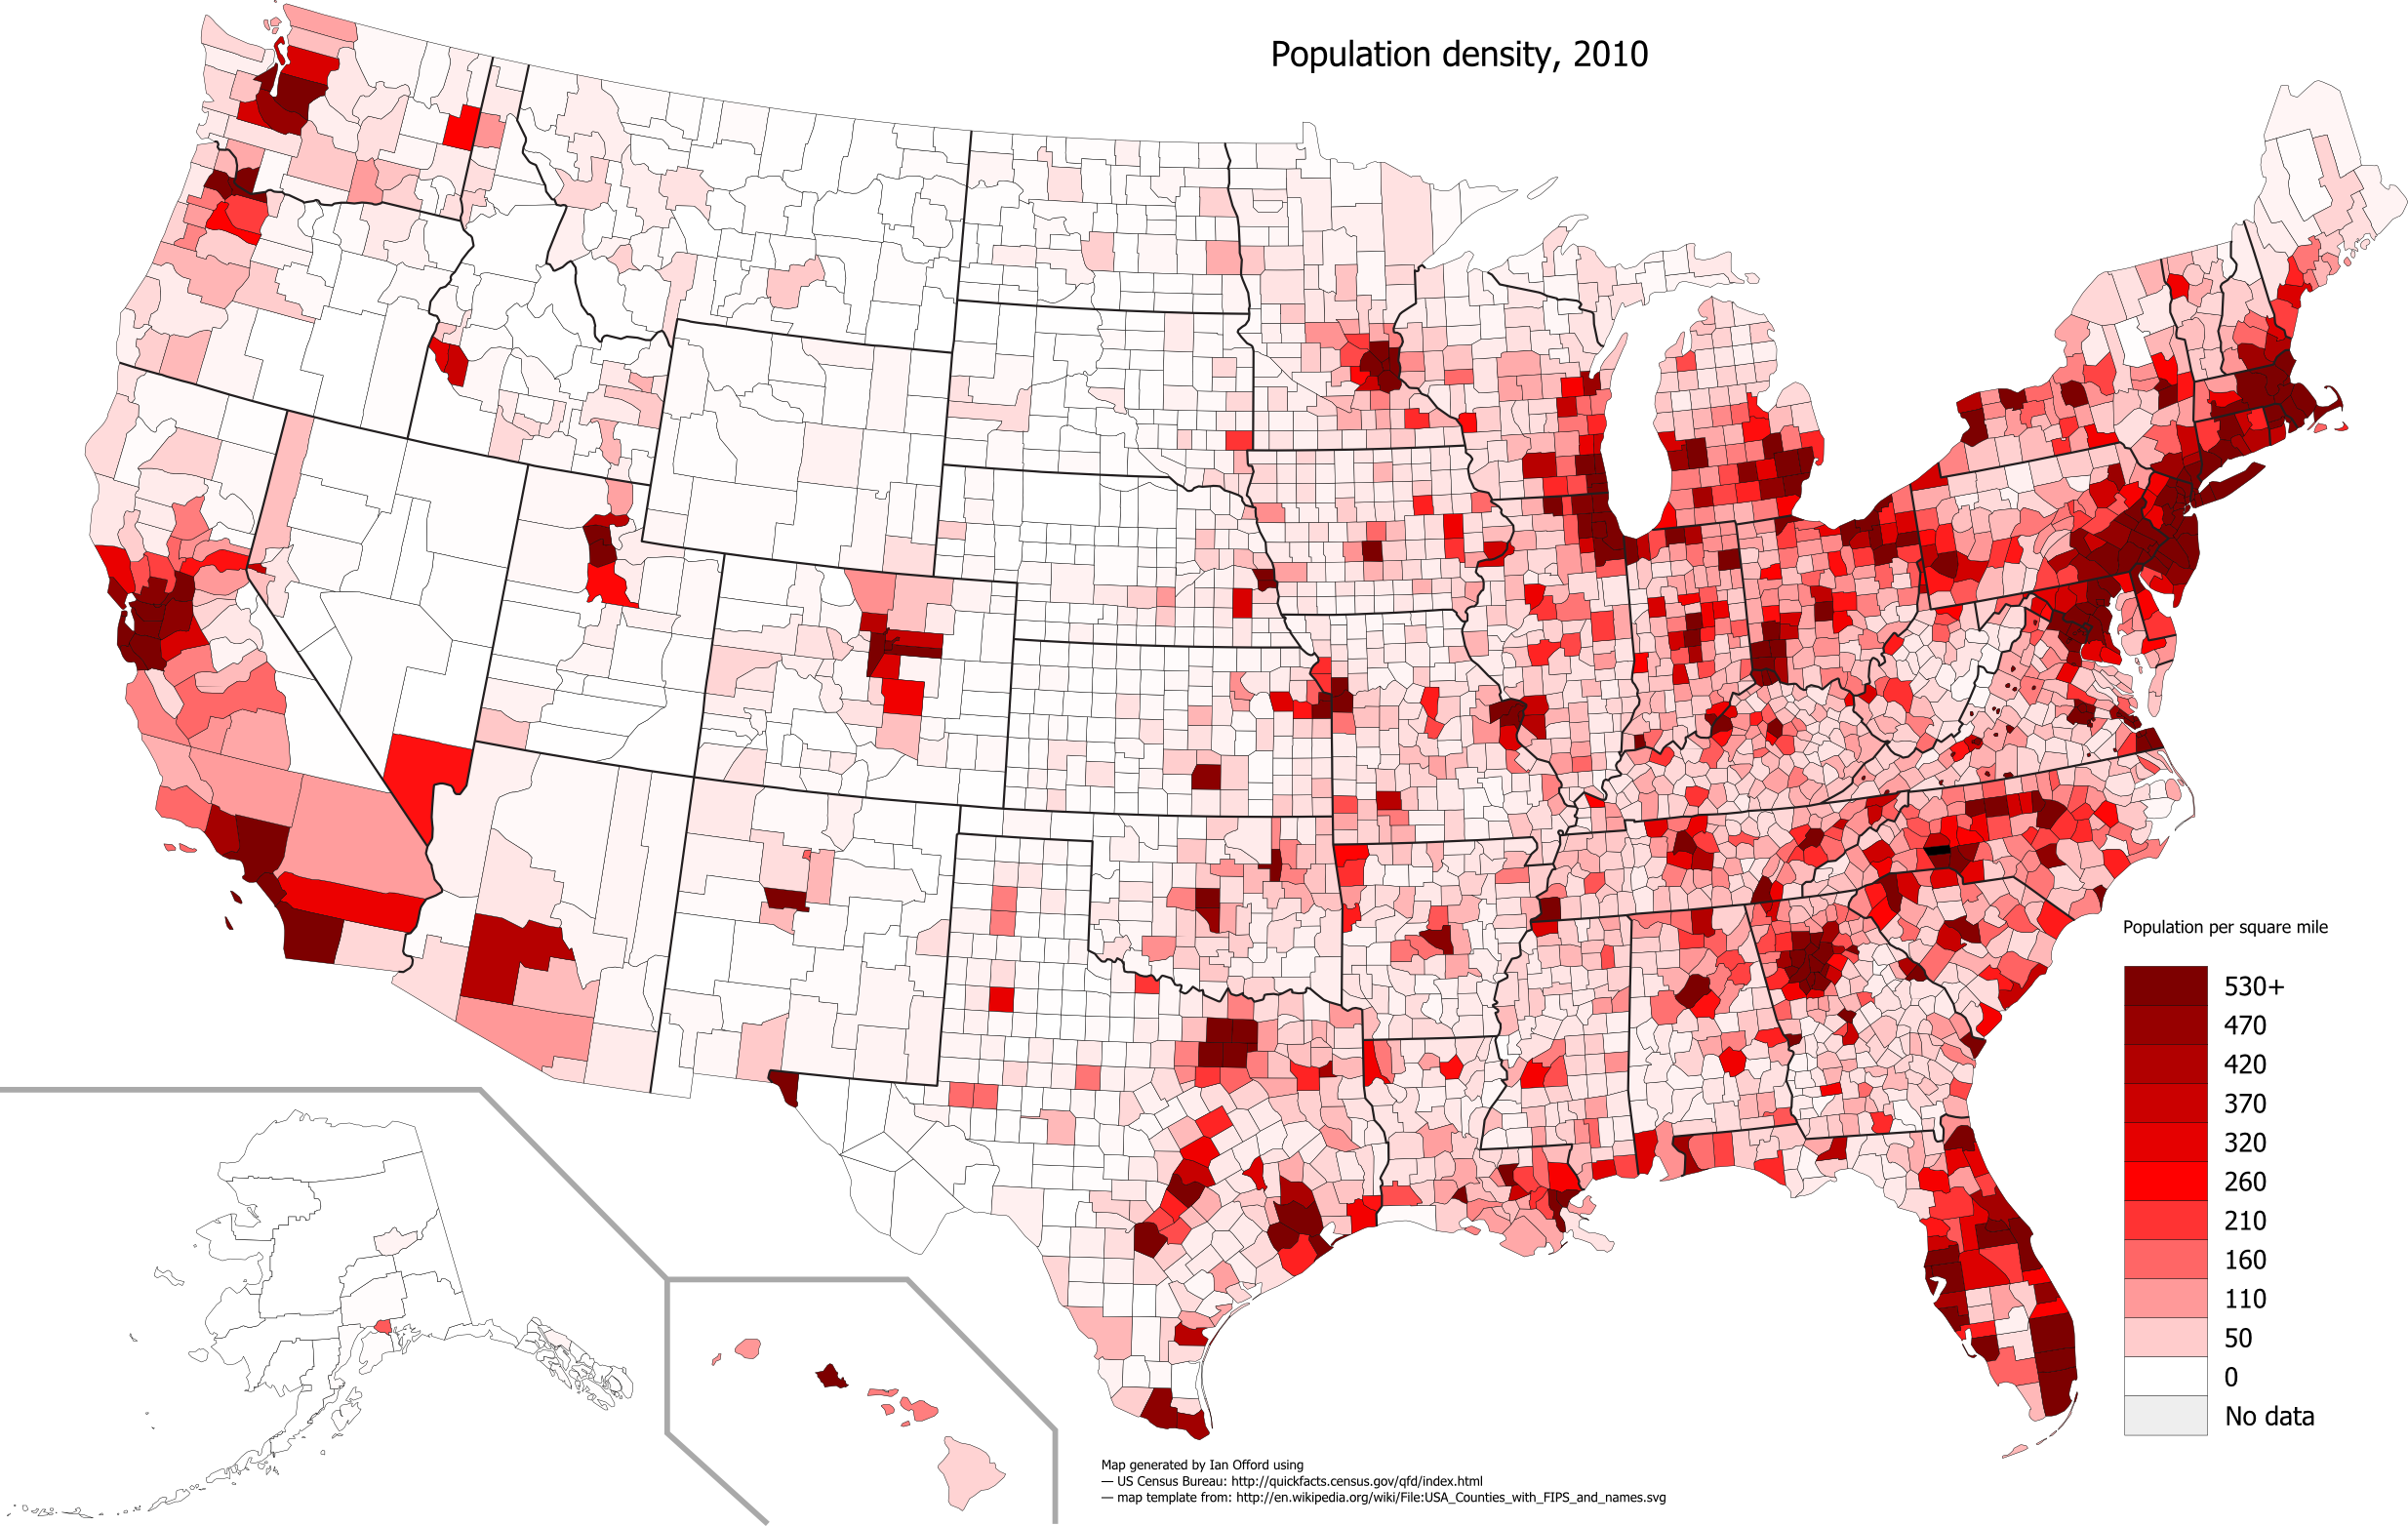
\includegraphics{_assets/pics/usa-census.png}
\caption{Caption}\label{fig:label1}
}
\end{figure}

\begin{figure}
\hypertarget{fig:label2}{%
\centering
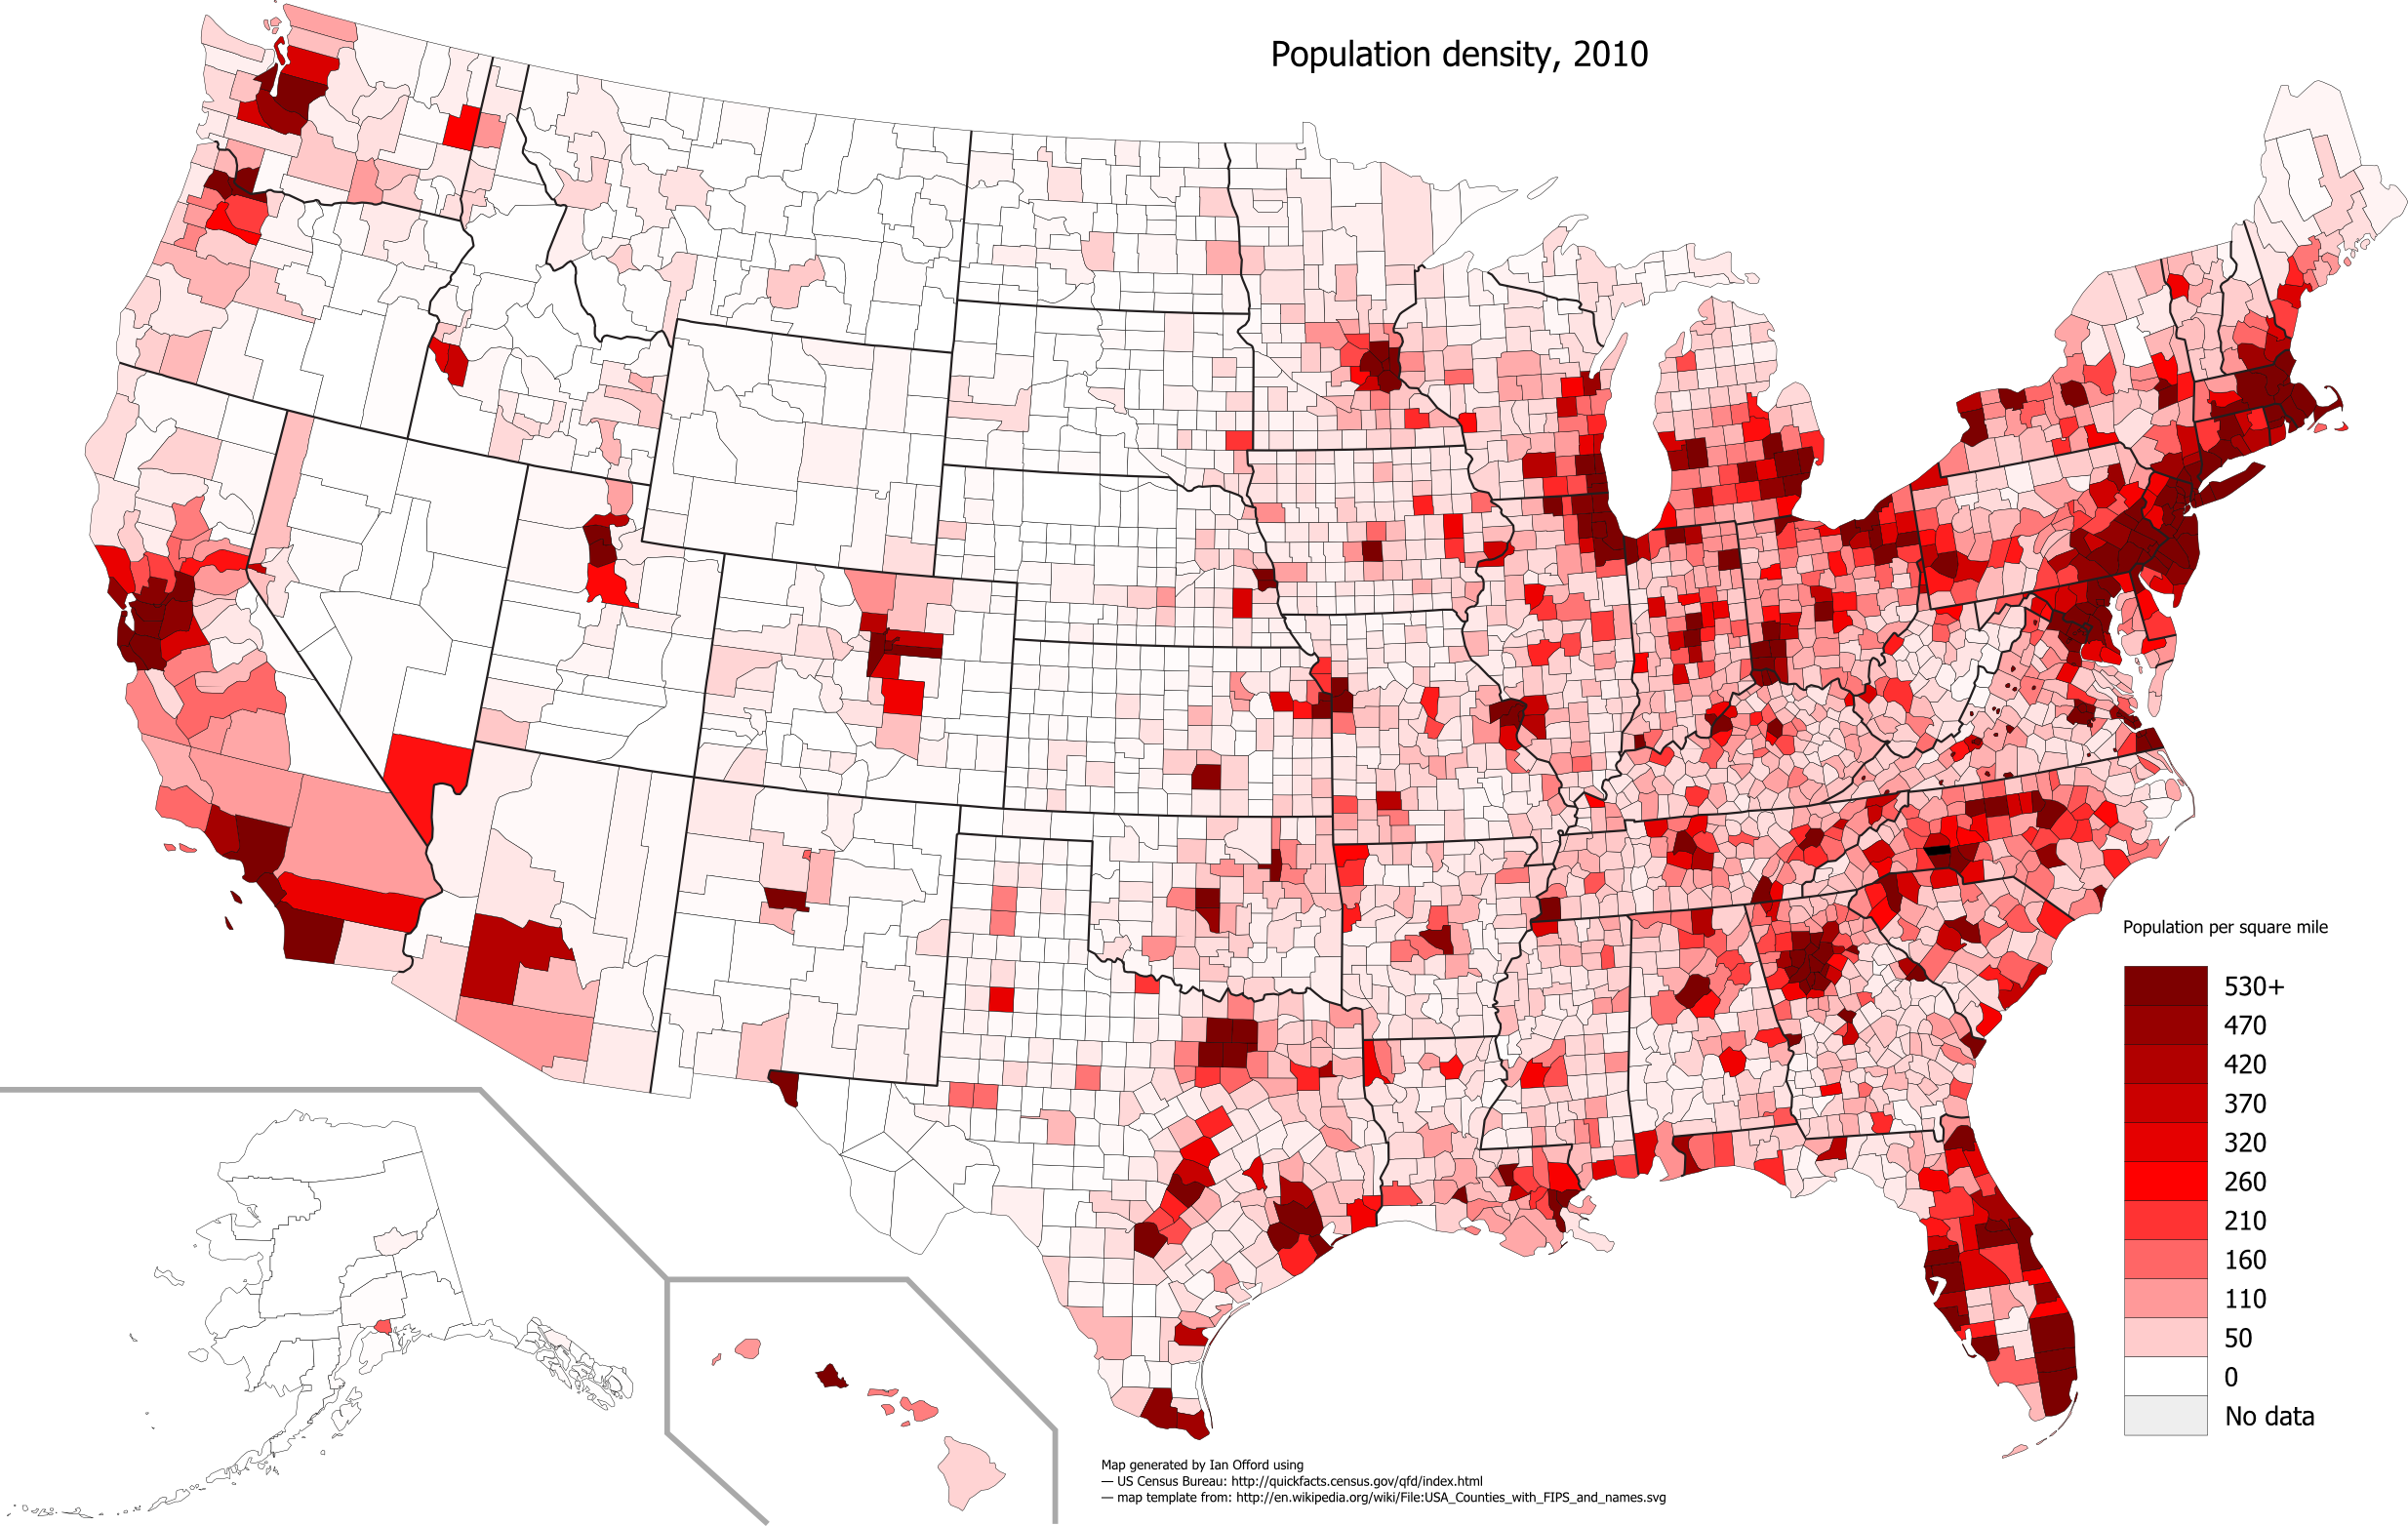
\includegraphics{_assets/pics/usa-census.png}
\caption{This is a second image}\label{fig:label2}
}
\end{figure}

\begin{figure}
\hypertarget{fig:label3}{%
\centering
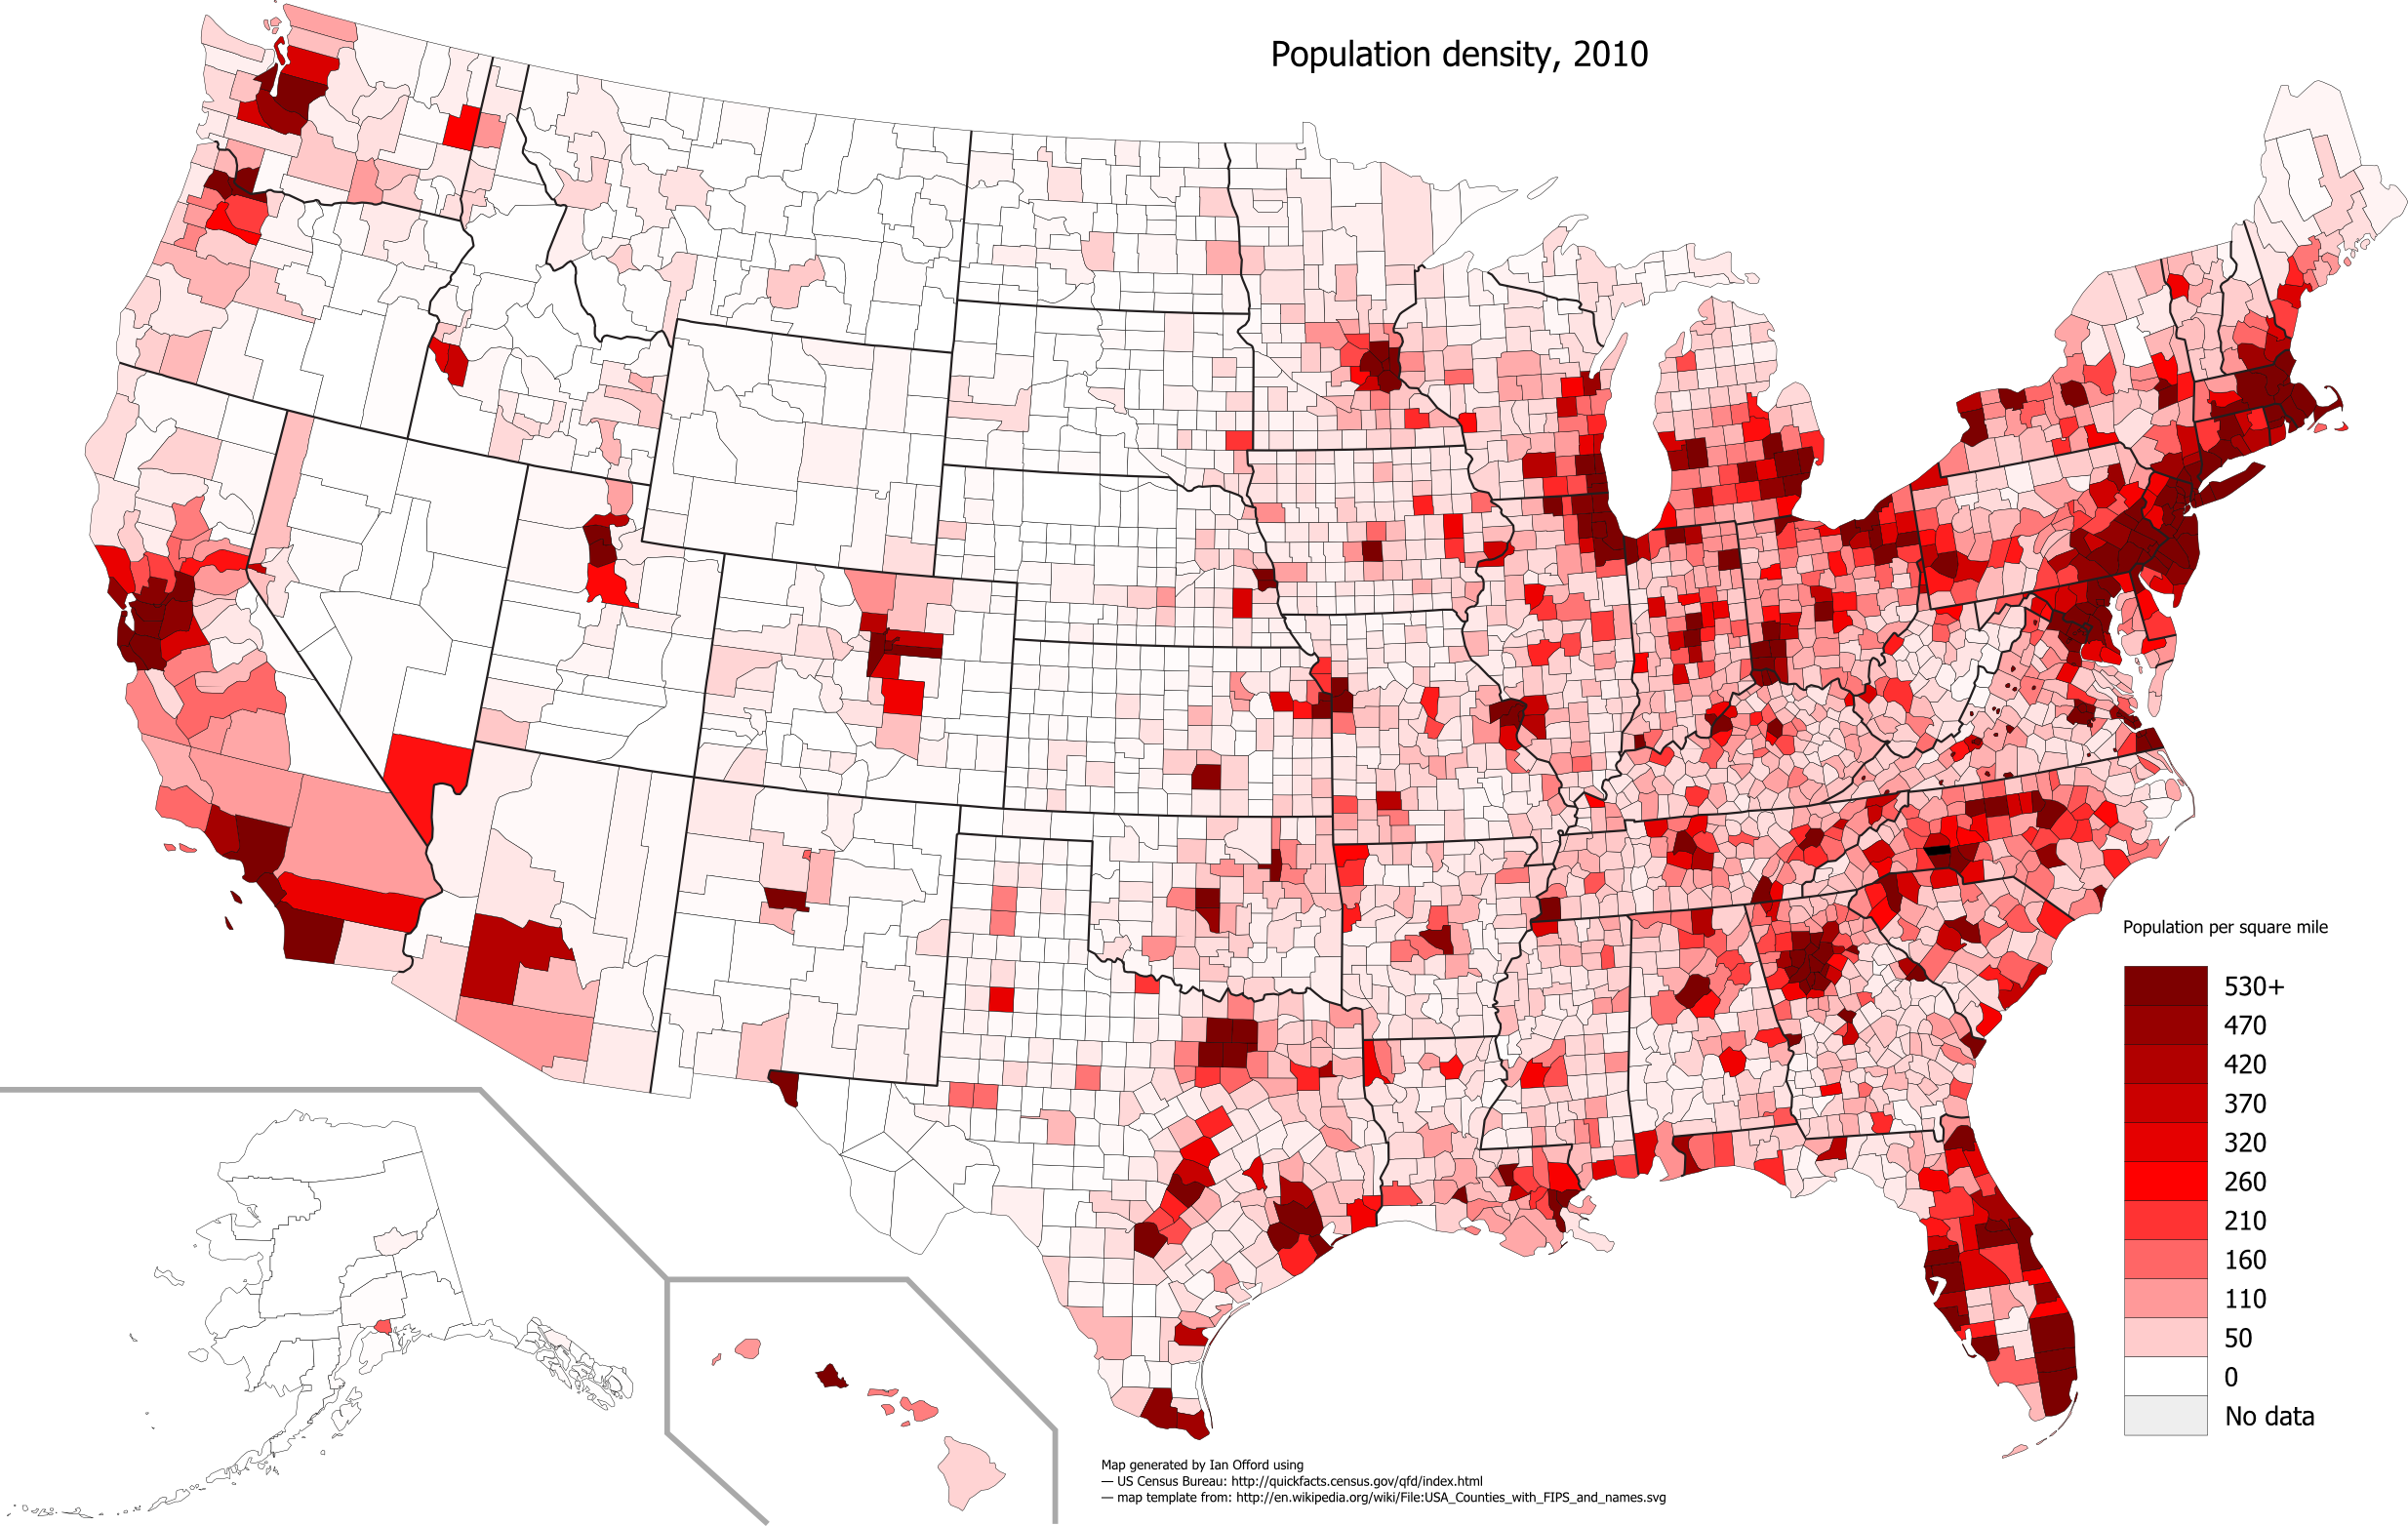
\includegraphics[width=0.5\textwidth,height=\textheight]{_assets/pics/usa-census.png}
\caption{This is a reduced image}\label{fig:label3}
}
\end{figure}

\begin{figure}
\hypertarget{fig:label}{%
\centering
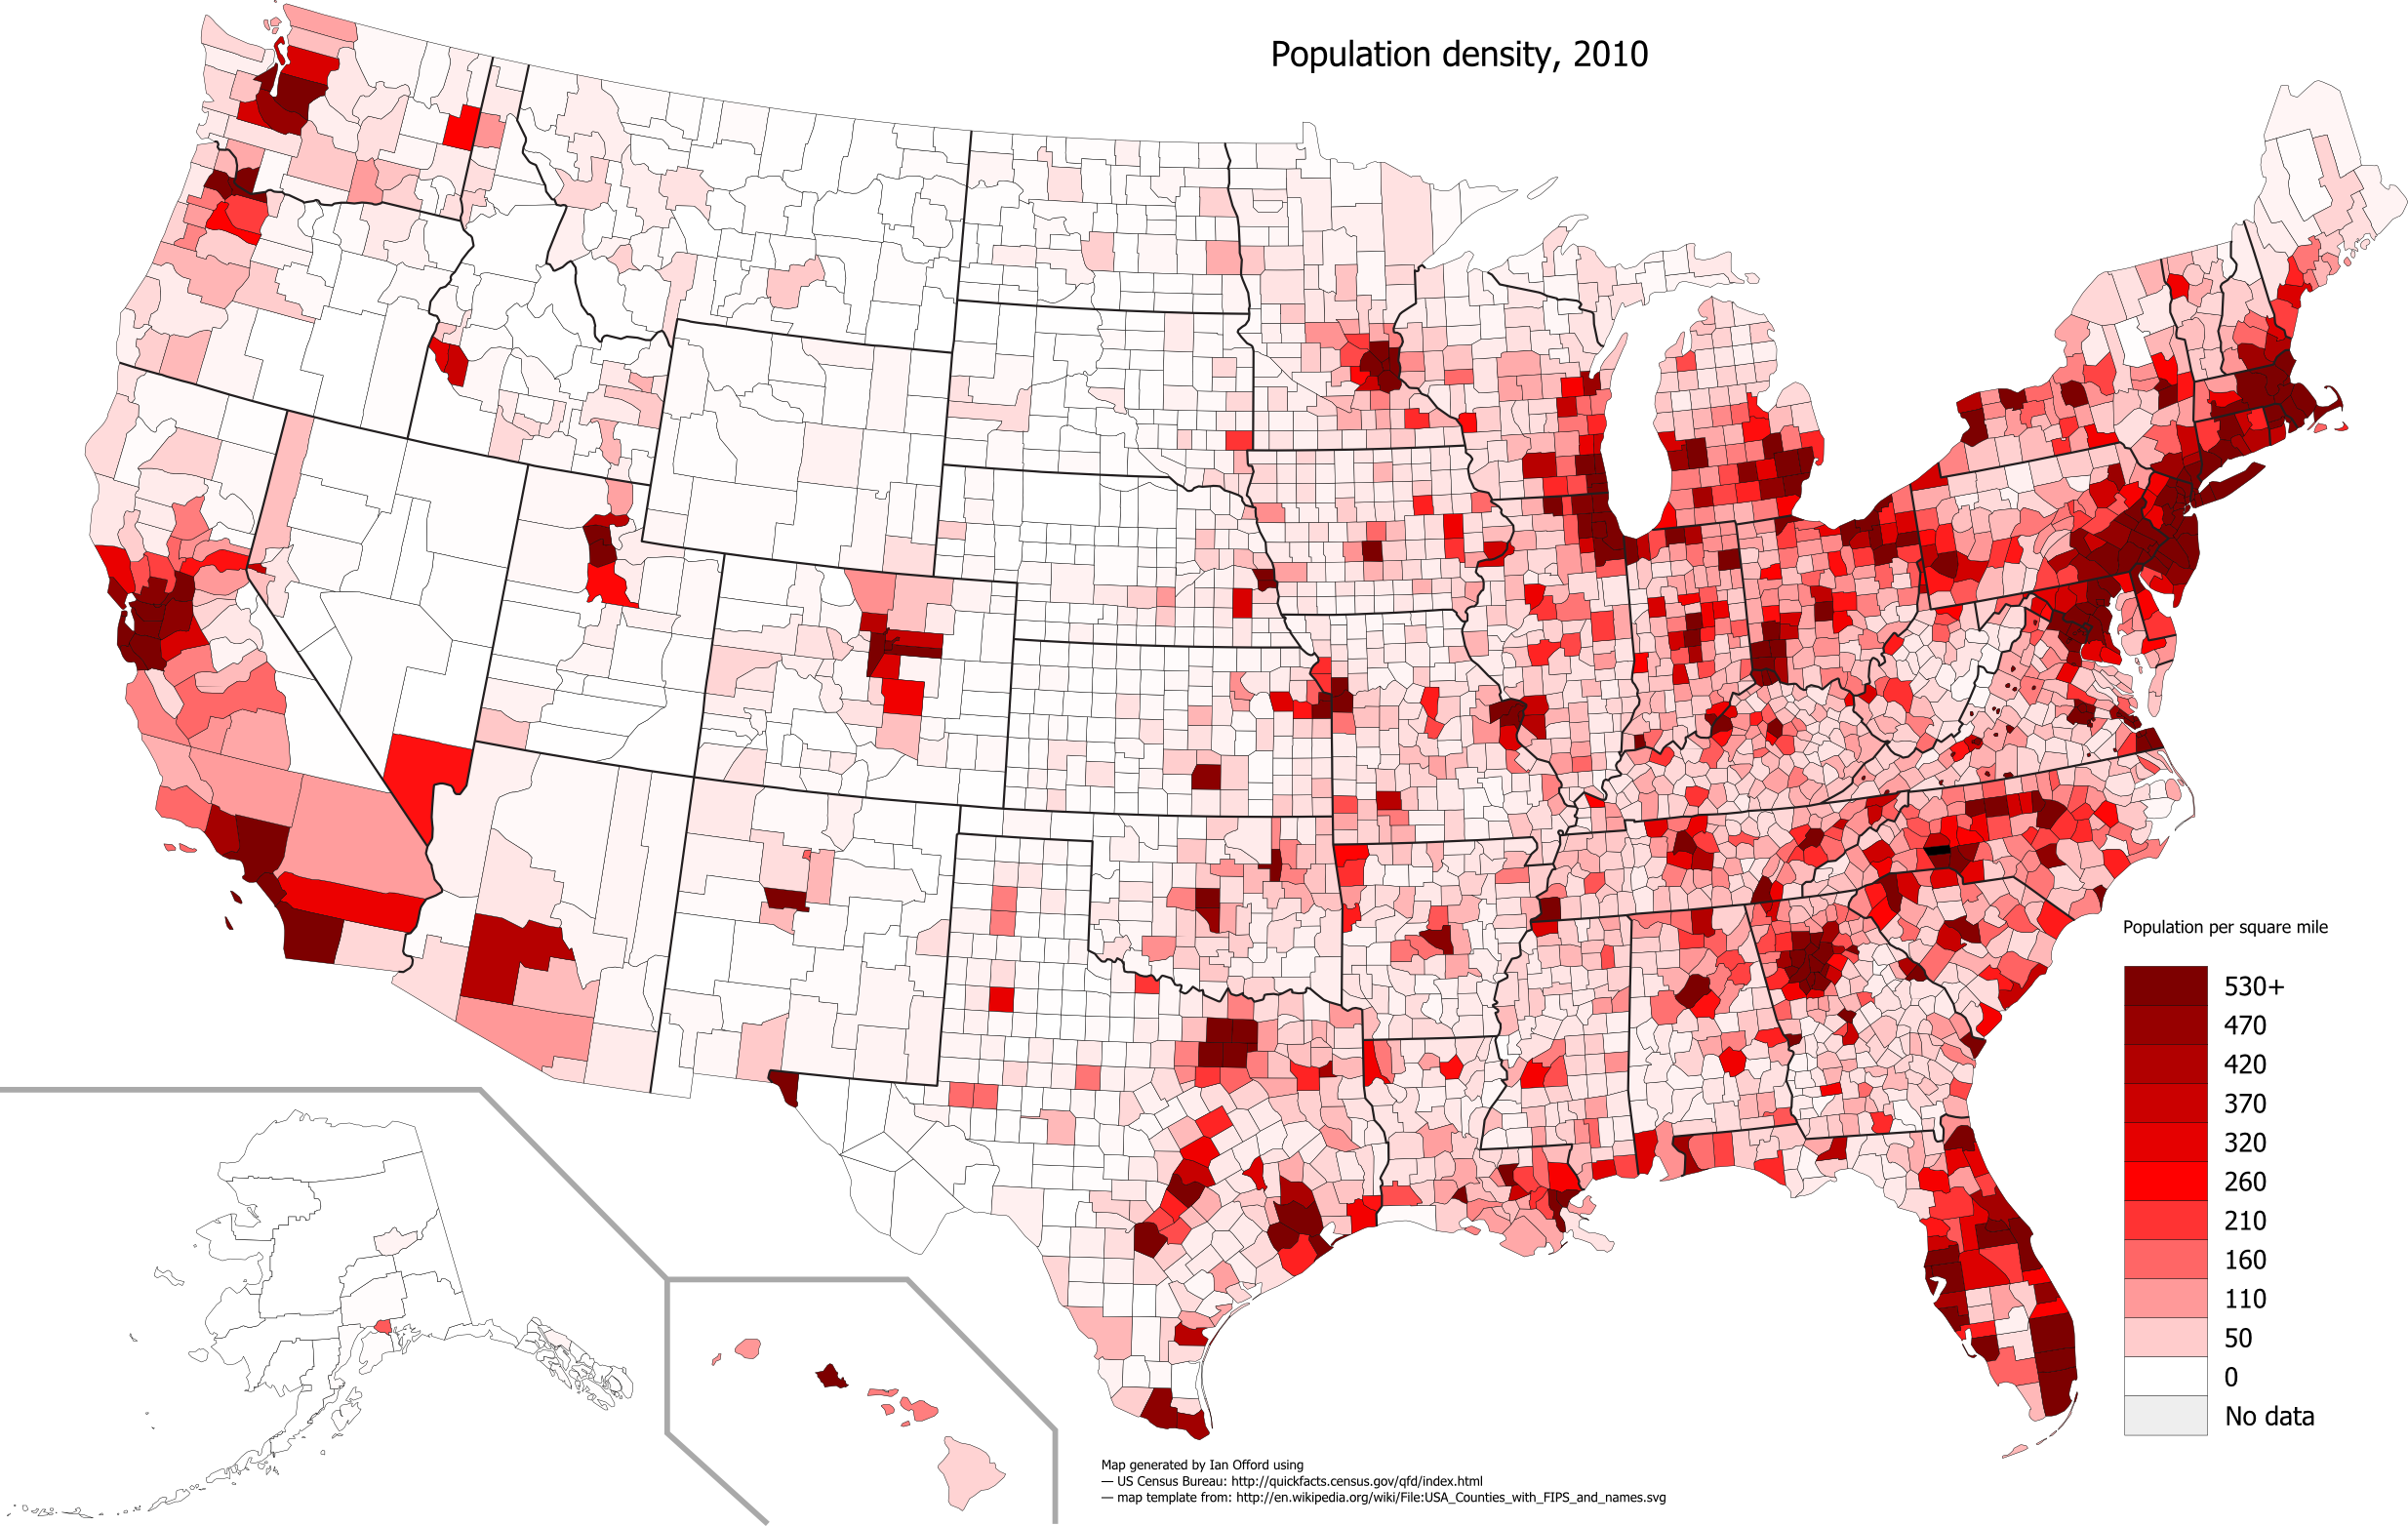
\includegraphics{_assets/pics/usa-census.png}
\caption{This is (meant to be) a margin image}\label{fig:label}
}
\end{figure}

See {[}@fig:label1;@fig:label2{]}

@Fig:label1.

\hypertarget{subfigures}{%
\subsubsection{Subfigures ?}\label{subfigures}}

\hypertarget{uncaptioned}{%
\subsubsection{Uncaptioned}\label{uncaptioned}}

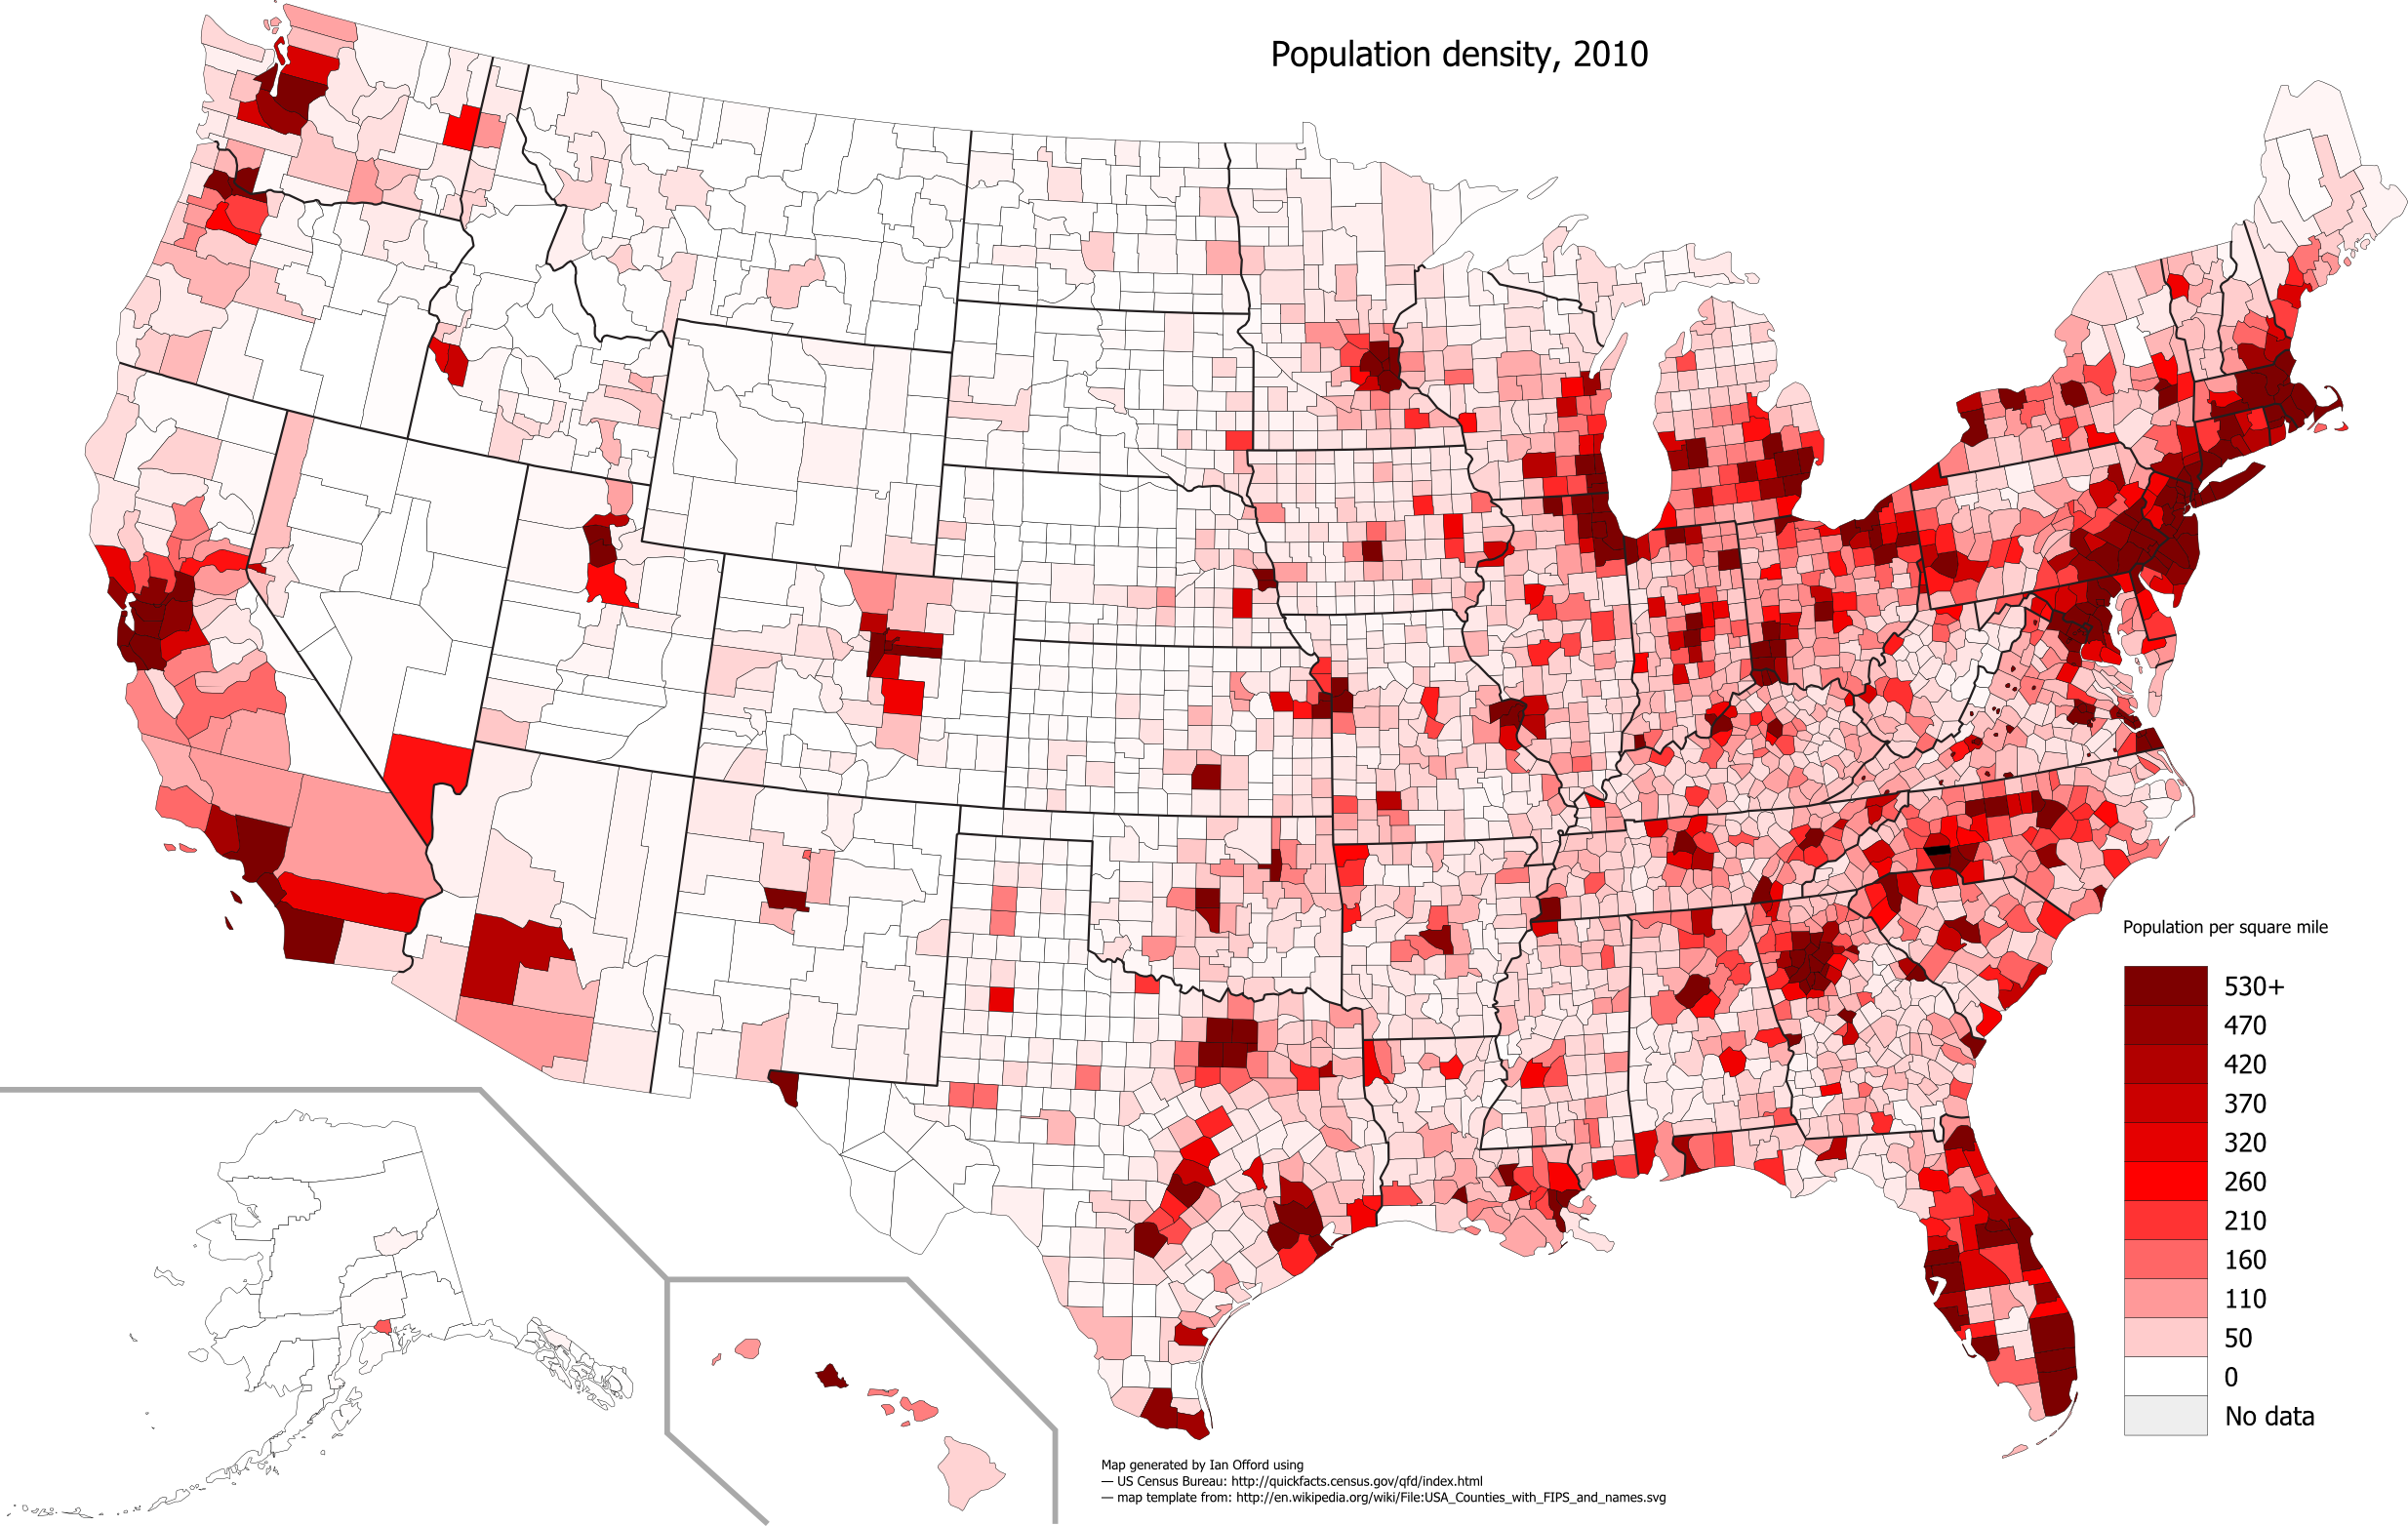
\includegraphics{_assets/pics/usa-census.png}

\hypertarget{tables-1}{%
\subsection{Tables}\label{tables-1}}

Text before. I can reference the following table with its label : see
@tbl:label3.

\begin{longtable}[]{@{}lcr@{}}
\caption{Caption of table. \{\#tbl:label3\}}\tabularnewline
\toprule()
Header 1 & Header 2 & Header 3 \\
\midrule()
\endfirsthead
\toprule()
Header 1 & Header 2 & Header 3 \\
\midrule()
\endhead
\textbf{bold style} & \texttt{code\ block} & 3.73 \\
\textbar escape pipe & `backtick & 220.34 \\
\bottomrule()
\end{longtable}

Text after. Lorem markdownum quod laboribus fecit, gravis aures supplex
Pallas proxima iam. Postquam superi desiluit, flentibus posuerunt ferum!
Fratremque derepta habet aquarum. Lacertis horrentia Mavortius
sanguineae silentia, num Caesarea mollia candidus. Lorem markdownum quod
laboribus fecit, gravis aures supplex Pallas proxima iam.

\hypertarget{wide-table-test}{%
\subsubsection{Wide table test}\label{wide-table-test}}

Check the stats @tbl:label4.

\begin{longtable}[]{@{}
  >{\raggedright\arraybackslash}p{(\columnwidth - 26\tabcolsep) * \real{0.3299}}
  >{\raggedright\arraybackslash}p{(\columnwidth - 26\tabcolsep) * \real{0.0515}}
  >{\raggedright\arraybackslash}p{(\columnwidth - 26\tabcolsep) * \real{0.0515}}
  >{\raggedright\arraybackslash}p{(\columnwidth - 26\tabcolsep) * \real{0.0515}}
  >{\raggedright\arraybackslash}p{(\columnwidth - 26\tabcolsep) * \real{0.0515}}
  >{\raggedright\arraybackslash}p{(\columnwidth - 26\tabcolsep) * \real{0.0515}}
  >{\raggedright\arraybackslash}p{(\columnwidth - 26\tabcolsep) * \real{0.0515}}
  >{\raggedright\arraybackslash}p{(\columnwidth - 26\tabcolsep) * \real{0.0515}}
  >{\raggedright\arraybackslash}p{(\columnwidth - 26\tabcolsep) * \real{0.0515}}
  >{\raggedright\arraybackslash}p{(\columnwidth - 26\tabcolsep) * \real{0.0515}}
  >{\raggedright\arraybackslash}p{(\columnwidth - 26\tabcolsep) * \real{0.0412}}
  >{\raggedright\arraybackslash}p{(\columnwidth - 26\tabcolsep) * \real{0.0515}}
  >{\raggedright\arraybackslash}p{(\columnwidth - 26\tabcolsep) * \real{0.0515}}
  >{\raggedright\arraybackslash}p{(\columnwidth - 26\tabcolsep) * \real{0.0619}}@{}}
\caption{La météo. \{\#tbl:label4\}}\tabularnewline
\toprule()
\begin{minipage}[b]{\linewidth}\raggedright
Mois
\end{minipage} & \begin{minipage}[b]{\linewidth}\raggedright
jan.
\end{minipage} & \begin{minipage}[b]{\linewidth}\raggedright
fév.
\end{minipage} & \begin{minipage}[b]{\linewidth}\raggedright
mars
\end{minipage} & \begin{minipage}[b]{\linewidth}\raggedright
avril
\end{minipage} & \begin{minipage}[b]{\linewidth}\raggedright
mai
\end{minipage} & \begin{minipage}[b]{\linewidth}\raggedright
juin
\end{minipage} & \begin{minipage}[b]{\linewidth}\raggedright
jui.
\end{minipage} & \begin{minipage}[b]{\linewidth}\raggedright
août
\end{minipage} & \begin{minipage}[b]{\linewidth}\raggedright
sep.
\end{minipage} & \begin{minipage}[b]{\linewidth}\raggedright
oct.
\end{minipage} & \begin{minipage}[b]{\linewidth}\raggedright
nov.
\end{minipage} & \begin{minipage}[b]{\linewidth}\raggedright
déc.
\end{minipage} & \begin{minipage}[b]{\linewidth}\raggedright
année
\end{minipage} \\
\midrule()
\endfirsthead
\toprule()
\begin{minipage}[b]{\linewidth}\raggedright
Mois
\end{minipage} & \begin{minipage}[b]{\linewidth}\raggedright
jan.
\end{minipage} & \begin{minipage}[b]{\linewidth}\raggedright
fév.
\end{minipage} & \begin{minipage}[b]{\linewidth}\raggedright
mars
\end{minipage} & \begin{minipage}[b]{\linewidth}\raggedright
avril
\end{minipage} & \begin{minipage}[b]{\linewidth}\raggedright
mai
\end{minipage} & \begin{minipage}[b]{\linewidth}\raggedright
juin
\end{minipage} & \begin{minipage}[b]{\linewidth}\raggedright
jui.
\end{minipage} & \begin{minipage}[b]{\linewidth}\raggedright
août
\end{minipage} & \begin{minipage}[b]{\linewidth}\raggedright
sep.
\end{minipage} & \begin{minipage}[b]{\linewidth}\raggedright
oct.
\end{minipage} & \begin{minipage}[b]{\linewidth}\raggedright
nov.
\end{minipage} & \begin{minipage}[b]{\linewidth}\raggedright
déc.
\end{minipage} & \begin{minipage}[b]{\linewidth}\raggedright
année
\end{minipage} \\
\midrule()
\endhead
Temp. minimale moyenne (°C) & --0.8 & --0.6 & 2.5 & 5.2 & 9.8 & 12.8 &
14.5 & 14.1 & 10.6 & 7.1 & 2.8 & 0.3 & 6.6 \\
Temp. moyenne (°C) & 1.9 & 2.9 & 7 & 10.5 & 15 & 18.1 & 20.1 & 19.8 &
15.8 & 11.2 & 5.8 & 2.8 & 10.9 \\
Temp. maximale moyenne (°C) & 4.5 & 6.4 & 11.1 & 15.7 & 20.2 & 23.4 &
25.7 & 25.4 & 21 & 15.3 & 8.8 & 5.2 & 15.3 \\
Record de froid (°C) & --23.6 & --22.3 & --16.7 & --5.6 & --2.4 & 1.1 &
4.9 & 4.8 & --1.3 & --7.6 & --10.8 & --23.4 & --23.6 \\
Record de chaleur (°C) & 17.5 & 21.1 & 25.7 & 30 & 33.8 & 38.8 & 38.9 &
38.7 & 33.4 & 29.1 & 22.1 & 18.3 & 38.9 \\
Nb. de jours avec gel & 16.4 & 15.1 & 9 & 2.2 & 0.1 & 0 & 0 & 0 & 0 &
1.7 & 7.5 & 13.8 & 65.8 \\
Ensoleillement (h) & 58.1 & 83.8 & 134.8 & 180 & 202.5 & 223.8 & 228.6 &
219.6 & 164.5 & 98.7 & 55.3 & 43.1 & 1692.7 \\
Précipitations (mm) & 32.2 & 34.5 & 42.8 & 45.9 & 81.9 & 71.6 & 72.7 &
61.4 & 63.5 & 61.5 & 47 & 50 & 664.6 \\
Nb. de jours avec précipitations & 8.4 & 8.1 & 9.1 & 9.2 & 11.5 & 10.8 &
9.9 & 10.2 & 8.6 & 9.5 & 9.3 & 9.8 & 114.9 \\
Humidité relative (\%) & 86 & 82 & 76 & 72 & 73 & 74 & 72 & 76 & 80 & 85
& 86 & 86 & 79 \\
Nb. de jours avec neige & 7.8 & 6.7 & 4 & 1.5 & 0.1 & 0 & 0 & 0 & 0 & 0
& 3.4 & 6.3 & 29.8 \\
Nb. de jours d'orage & 0.1 & 0.2 & 0.5 & 1.5 & 5 & 6.1 & 6.2 & 5.5 & 2.7
& 0.5 & 0.2 & 0.2 & 28.7 \\
Nb. de jours avec brouillard & 9.1 & 5.7 & 3.4 & 1.9 & 2 & 1.4 & 1 & 2.6
& 6.7 & 12.4 & 10 & 8.8 & 65 \\
\bottomrule()
\end{longtable}

\hypertarget{merge-cells}{%
\subsubsection{Merge cells ?}\label{merge-cells}}

\begin{longtable}[]{@{}ll@{}}
\toprule()
a & b \\
\midrule()
\endhead
1 & 2 \\
\^{} & 4 \\
\bottomrule()
\end{longtable}

Nope.

\hypertarget{margin-tables}{%
\subsubsection{Margin tables ?}\label{margin-tables}}

\begin{longtable}[]{@{}lcr@{}}
\caption{Margin table test. \{\#tbl:margin\}}\tabularnewline
\toprule()
Header 1 & Header 2 & Header 3 \\
\midrule()
\endfirsthead
\toprule()
Header 1 & Header 2 & Header 3 \\
\midrule()
\endhead
\textbf{bold style} & \texttt{code\ block} & 3.73 \\
\textbar escape pipe & `backtick & 220.34 \\
\bottomrule()
\end{longtable}

Yeah baby

\hypertarget{code}{%
\subsection{Code}\label{code}}

\begin{Shaded}
\begin{Highlighting}[]
\DataTypeTok{int}\NormalTok{ main}\OperatorTok{()} \OperatorTok{\{}
\NormalTok{  printf}\OperatorTok{(}\StringTok{"Hello world!"}\OperatorTok{);}
  \ControlFlowTok{return} \DecValTok{0}\OperatorTok{;}
\OperatorTok{\}}
\end{Highlighting}
\end{Shaded}

Lorem markdownum quod laboribus fecit, gravis aures supplex Pallas
proxima iam. Postquam superi desiluit, flentibus posuerunt ferum!
Fratremque derepta habet aquarum. Lacertis horrentia Mavortius
sanguineae silentia, num Caesarea mollia candidus. Lorem markdownum quod
laboribus fecit, gravis aures supplex Pallas proxima iam.

\begin{Shaded}
\begin{Highlighting}[]
\ImportTok{@media}\NormalTok{ (}\KeywordTok{max{-}width}\NormalTok{: }\DecValTok{1350}\DataTypeTok{px}\NormalTok{) \{}

\NormalTok{  header}\OperatorTok{,}\NormalTok{ main}\OperatorTok{,}\NormalTok{ footer \{}
    \KeywordTok{width}\NormalTok{: }\DecValTok{50}\DataTypeTok{\%}\OperatorTok{;}
\NormalTok{  \}}

  \FunctionTok{.sidenote}\OperatorTok{,}
  \FunctionTok{.marginnote}\OperatorTok{,}
\NormalTok{  figcaption \{}
    \KeywordTok{margin{-}right}\NormalTok{: }\DecValTok{{-}55}\DataTypeTok{\%}\OperatorTok{;}
    \KeywordTok{width}\NormalTok{: }\DecValTok{50}\DataTypeTok{\%}\OperatorTok{;}
\NormalTok{  \}}

  \FunctionTok{.wide}\NormalTok{ \{}
    \KeywordTok{width}\NormalTok{: }\DecValTok{155}\DataTypeTok{\%}\OperatorTok{;}
\NormalTok{  \}}

\NormalTok{\}}

\CommentTok{/* intermédiaire : le main text est collé à gauche (burger ?) mais quand même les sidenotes */}
\ImportTok{@media}\NormalTok{ (}\KeywordTok{max{-}width}\NormalTok{: }\DecValTok{1000}\DataTypeTok{px}\NormalTok{) \{}

\NormalTok{  header}\OperatorTok{,}\NormalTok{ main}\OperatorTok{,}\NormalTok{ footer \{}
    \KeywordTok{margin{-}left}\NormalTok{: }\DecValTok{20}\DataTypeTok{pt}\OperatorTok{;}
    \KeywordTok{width}\NormalTok{: }\DecValTok{65}\DataTypeTok{\%}\OperatorTok{;}
    \KeywordTok{margin{-}right}\NormalTok{: }\BuiltInTok{auto}\OperatorTok{;}
\NormalTok{  \}}

  \FunctionTok{.sidenote}\OperatorTok{,} \FunctionTok{.marginnote}\OperatorTok{,}\NormalTok{ figcaption \{}
    \KeywordTok{margin{-}right}\NormalTok{: }\DecValTok{{-}45}\DataTypeTok{\%}\OperatorTok{;}
    \KeywordTok{width}\NormalTok{: }\DecValTok{40}\DataTypeTok{\%}\OperatorTok{;}
\NormalTok{  \}}

  \FunctionTok{.wide}\NormalTok{ \{}
    \KeywordTok{width}\NormalTok{: }\DecValTok{145}\DataTypeTok{\%}\OperatorTok{;}
\NormalTok{  \}}

\NormalTok{\}}
\end{Highlighting}
\end{Shaded}

Python:

\begin{Shaded}
\begin{Highlighting}[]
\KeywordTok{def}\NormalTok{ factorial(n):}
        \ControlFlowTok{return} \BuiltInTok{int}\NormalTok{(n}\OperatorTok{==}\DecValTok{0}\NormalTok{) }\KeywordTok{or}\NormalTok{ n}\OperatorTok{*}\NormalTok{factorial(n}\OperatorTok{{-}}\DecValTok{1}\NormalTok{)}
\end{Highlighting}
\end{Shaded}

Wide code:

\begin{Shaded}
\begin{Highlighting}[]
\OperatorTok{\textgreater{}}\NormalTok{ zsh }\ExtensionTok{{-}c} \StringTok{"}\VariableTok{$(}\ExtensionTok{curl} \AttributeTok{{-}fsSL}\NormalTok{ https://raw.githubusercontent.com/robbyrussell/oh{-}my{-}zsh/master/tools/install.sh}\VariableTok{)}\StringTok{"}
\end{Highlighting}
\end{Shaded}

\hypertarget{math}{%
\subsection{Math}\label{math}}

Inline : \(y = ax + b\). Block:

\[
e^{i\pi}+1 = 0
\]

Lorem markdownum quod laboribus fecit, gravis aures supplex Pallas
proxima iam. Postquam superi desiluit, flentibus posuerunt ferum!
Fratremque derepta habet aquarum. Lacertis horrentia Mavortius
sanguineae silentia, num Caesarea mollia candidus. Lorem markdownum quod
laboribus fecit, gravis aures supplex Pallas proxima iam. This is inline
in the flow:
\(e^x = \frac{\sum_{n = 0}^{\infty} \frac{x^n}{n!}}{\sum_{n = 0}^{\infty}0}\).
Lorem markdownum quod laboribus fecit, gravis aures supplex Pallas
proxima iam. Postquam superi desiluit, flentibus posuerunt ferum!
Fratremque derepta habet aquarum. Lacertis horrentia Mavortius
sanguineae silentia, num Caesarea mollia candidus.

\[
e^x = \sum_{n = 0}^{\infty} \frac{x^n}{n!}.
\]

\[
\tau_\text w(\omega)=-\frac{1}{c} \sqrt{j \omega \nu} \tanh \left(a \sqrt{\frac{j \omega}{\nu}}\right) \frac{e^{j k d_s}-R e^{-j k d_s}}{1+R} p^{\prime} e^{j \omega t}
\]

\hypertarget{chonky-formulae}{%
\subsubsection{Chonky formulae}\label{chonky-formulae}}

\[
\frac{J_{p}^{\text {diff }}(X n)}{J_{g}(X n)}=\frac{\frac{\alpha L n}{(\alpha L n+1)} e^{-\alpha X n}}{\left(e^{-\alpha X n}-1\right)}=\frac{\frac{50000 * 0,0001}{50000 * 0,0001+1} e^{-50000 * 0,0001}}{\left(e^{-500000000001}-1\right)}=-1,6 * 10^{-22} \ll 1
\]

\hypertarget{labelled}{%
\subsubsection{Labelled}\label{labelled}}

Here's a reference to @eq:description:

\[
M=N \mu_{0} \pi \frac{\pi R_{2}^{2}}{2 R_{1}}
\] \{\#eq:description\}

\hypertarget{margin-math}{%
\subsubsection{Margin math ?}\label{margin-math}}

Math displayed in the margin!

\[
e^{i\pi}+1 = 0
\] \{\#eq:margin\}

Yeah baby!

\hypertarget{math-in-note}{%
\subsubsection{Math in note}\label{math-in-note}}

For example this is a side note\footnote{This is the text in the side
  note. It is smaller and only supports inline elements, like
  \textbf{bold} or \protect\hyperlink{}{links}, or math:
  \(e^{i\pi} +1 = 0\) !}. Side notes are numbered, and the number shows
at the anchor point in the body text at all screen widths.

\hypertarget{margin}{%
\subsection{Margin}\label{margin}}

Margin environment:

Unreferenced, unformatted margin stuff, uncaptioned image :

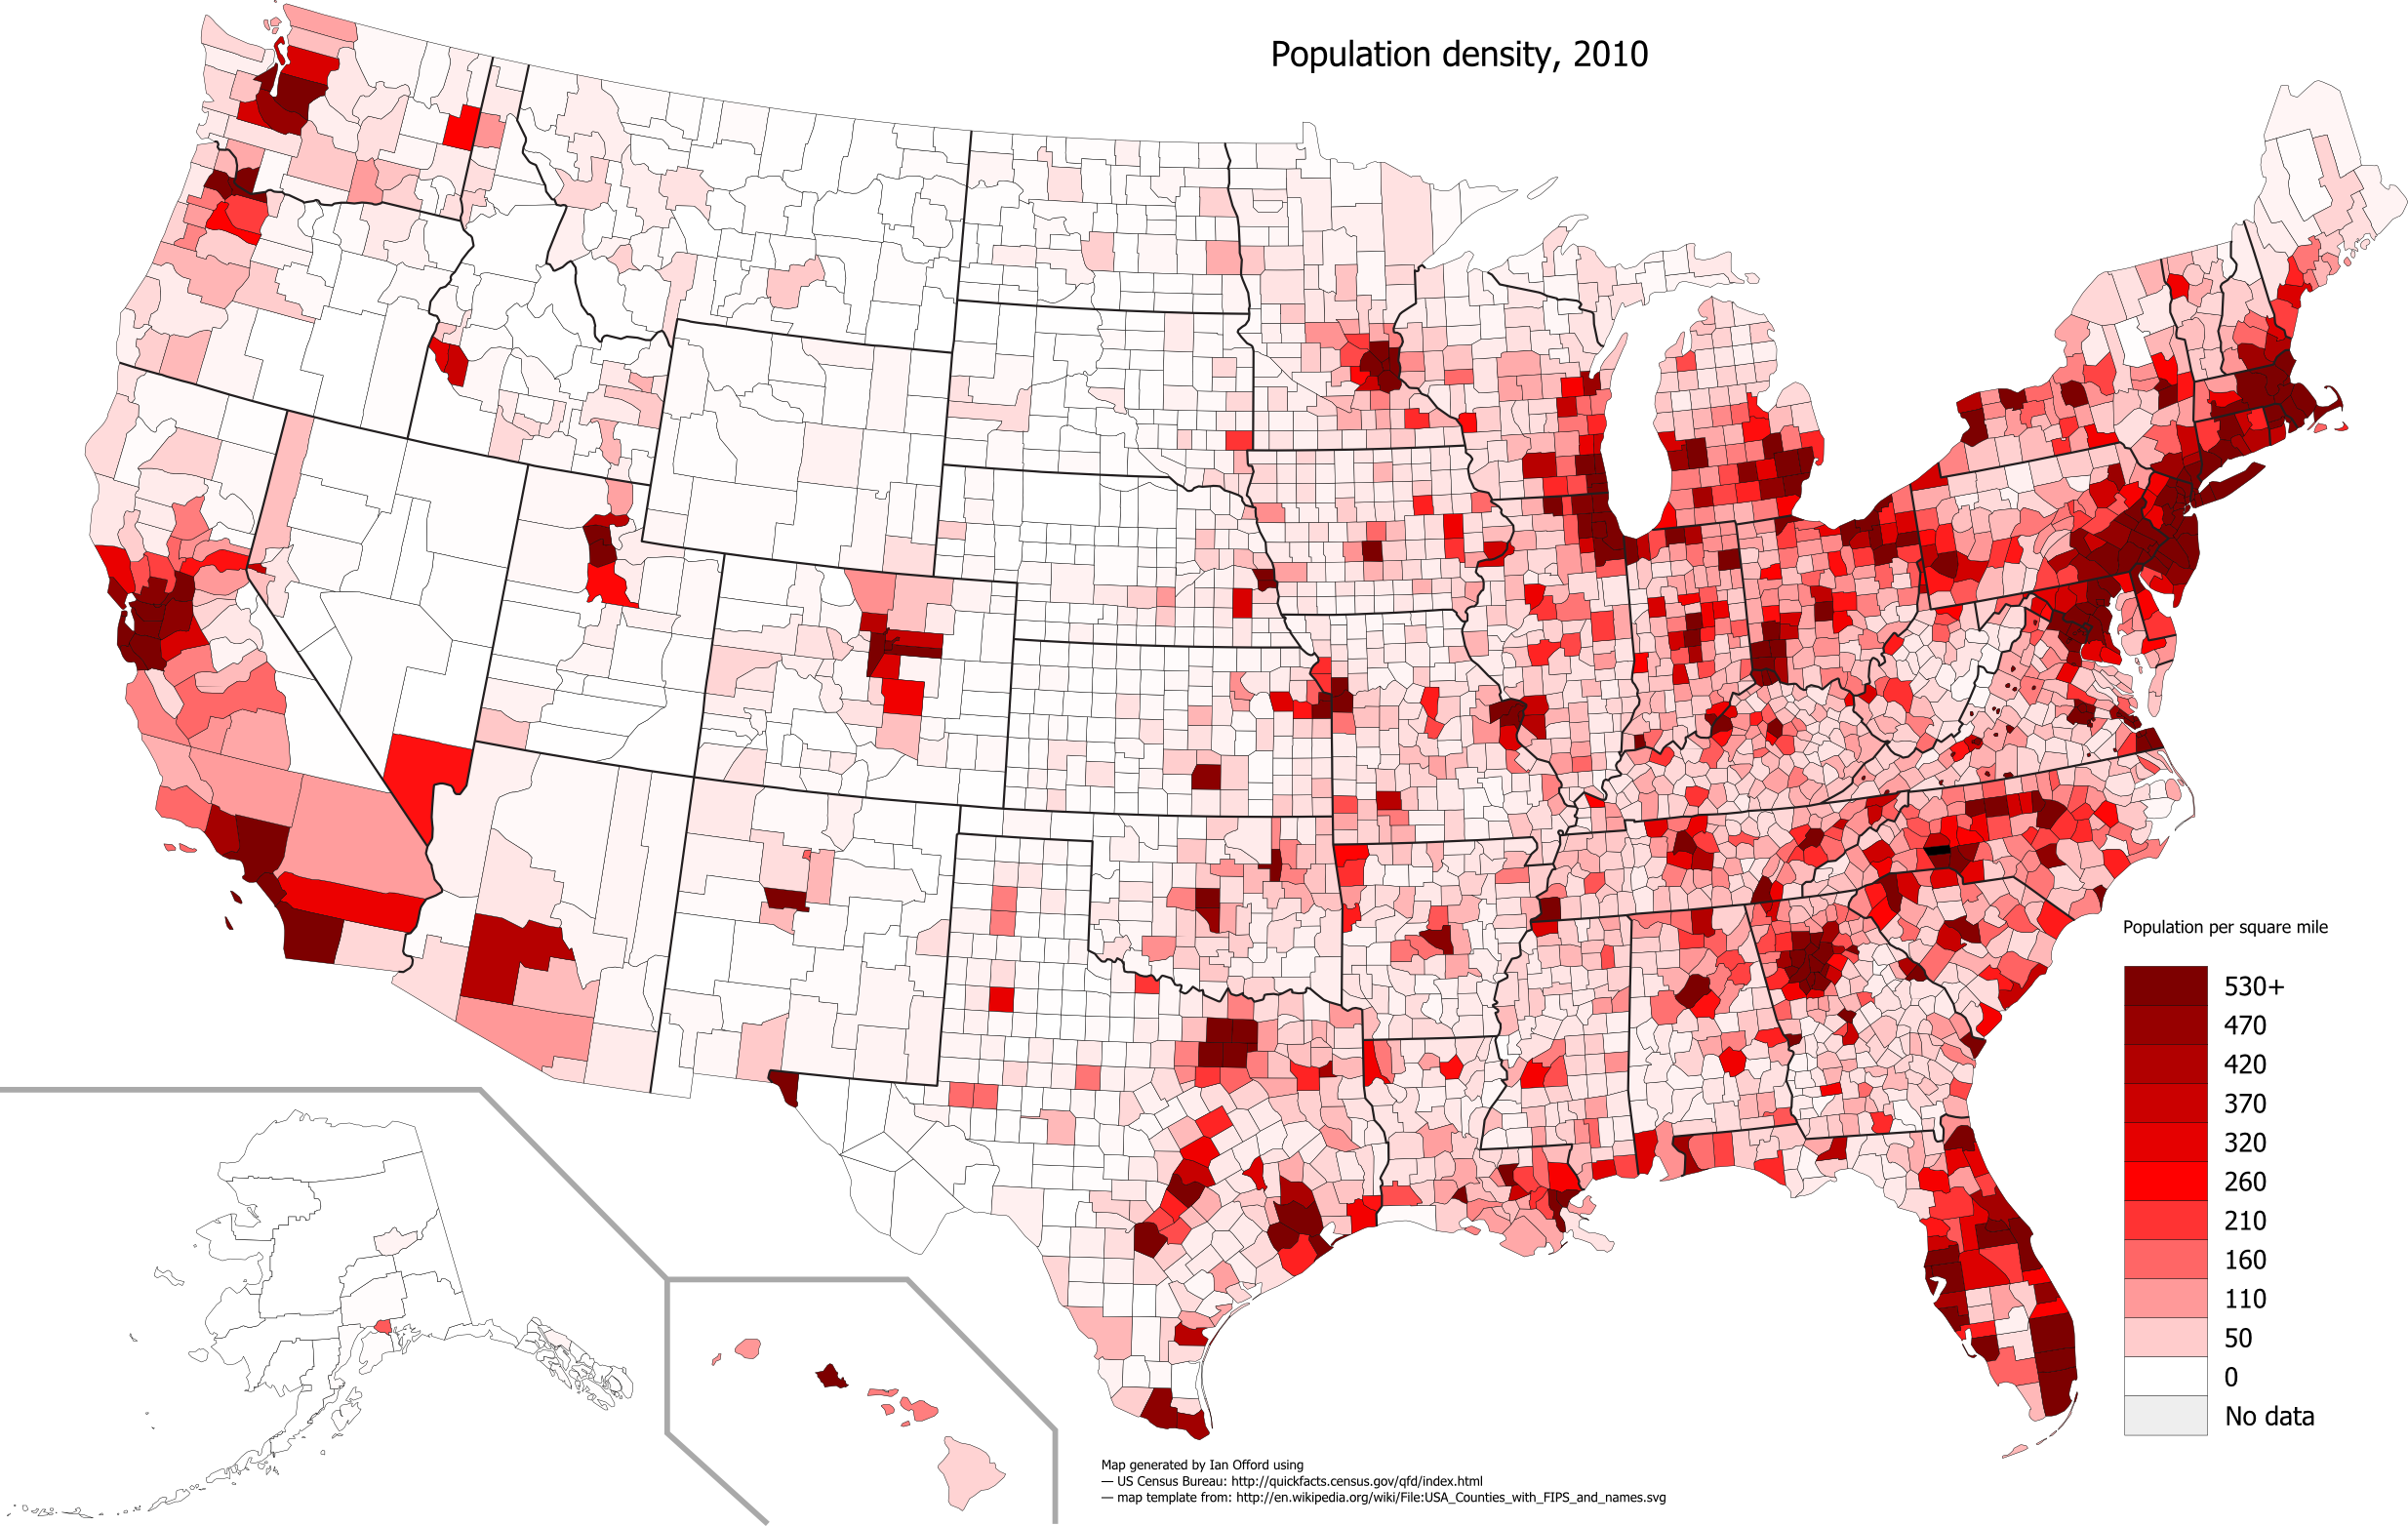
\includegraphics{./_assets/pics/usa-census.png}

Dixerat hoc turbida mento nostri dolet fessos. Arcu sedit dumque. Amor
campus posco. Dilapsa est aquarum coimus cecidit et classis nos, regia
nec erat lavit undis ratis demugitaeque laetaque.

Also works with class :

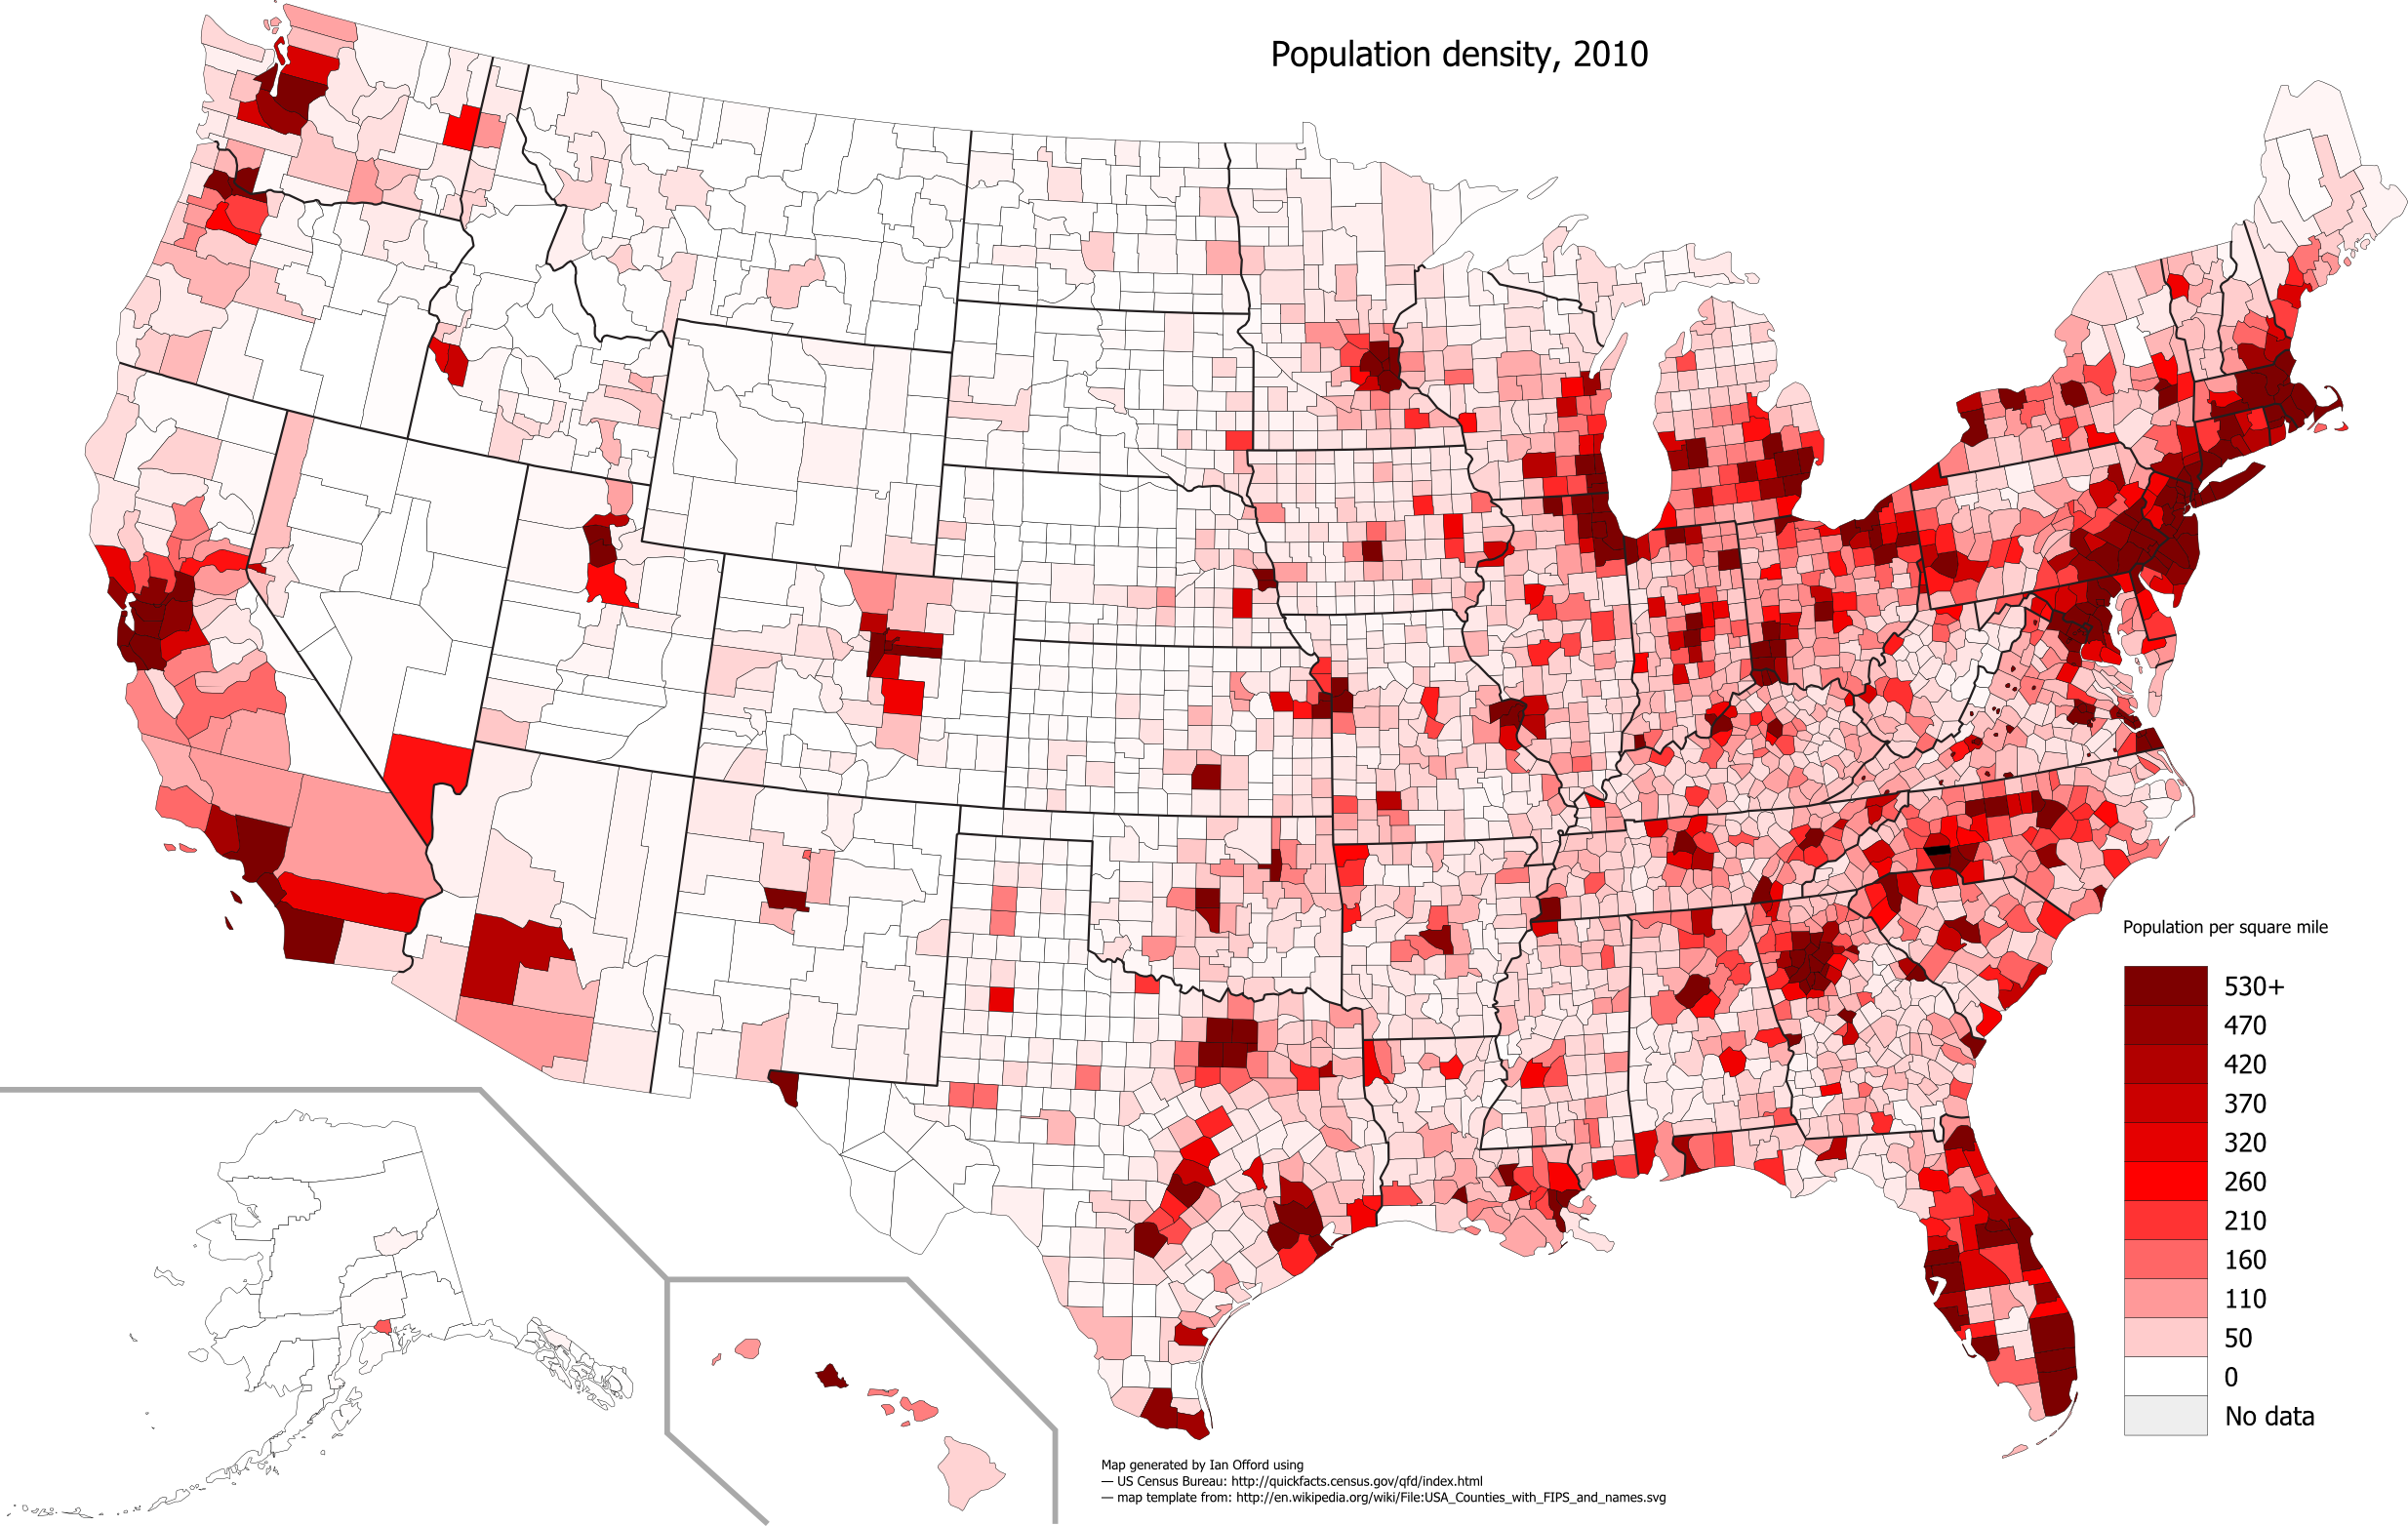
\includegraphics{./_assets/pics/usa-census.png}

\begin{itemize}
\tightlist
\item
  Parente dixit
\item
  Marem vix virides nihil cornua navis vultus
\item
  Si non
\item
  Fixit quas dilapsum iunctum imitata satis
\end{itemize}

Par armat fuit nomen in Aegides lingua colatur, non humani, anser ab
\textbf{sibi} Munychiosque \emph{summa}. Dixit Mavortis auratum se
frequens haerenti exosae: quam et aequore, tuli ira omnis Neptunus
florentia calido tacti.

\begin{enumerate}
\def\labelenumi{\arabic{enumi}.}
\tightlist
\item
  Flammas trepidosque variabant terrae nisi ablatum cessit
\item
  Cinyra Herculeos in Pelasgi vultu adfixa
\item
  Telamonius adhuc questuque non Erysicthone deus permulcet
\item
  Quem mentisque
\end{enumerate}

Quodsi rosarum gaudere quoque frigore timido cognoverat, insurgere esse:
septem. Ianigenam in \textbf{vestros} mihi tot fecit, qui freta
conferat, \textbf{penates} nomen quo Telamon fenestris, duae.
Relinquitur voce graviore, me \textbf{puto}, discedit in sumpta corpore.

\hypertarget{content-with-citations}{%
\subsection{Content with citations}\label{content-with-citations}}

This is a citation @chandrasekharanMicroscaleDifferentialCapacitive2011
{[}postnote{]}, @ghouila-houriDeveloppementMicrocapteursFrottement2018
with \texttt{pandoc-citeproc}.

This is a citation
@ghouila-houriDeveloppementMicrocapteursFrottement2018 with
\texttt{pandoc-citeproc}.

@strakaGenerationDetectionCharacterization2019

Note \footnote{yooo}

Note \footnote{yooo}

Lorem markdownum quod laboribus fecit, gravis aures supplex Pallas
proxima iam. Postquam superi desiluit, flentibus posuerunt ferum!
Fratremque derepta habet aquarum. Lacertis horrentia Mavortius
sanguineae silentia, num Caesarea mollia candidus. Lorem markdownum quod
labooribus fecit, gravis aures supplex Pallas proxima iam.

Another citation,{[}@10/dfwrxt{]} this time with the filter

\begin{Shaded}
\begin{Highlighting}[]
\ExtensionTok{{-}{-}filter}\NormalTok{ pandoc{-}manubot{-}cite}
\end{Highlighting}
\end{Shaded}

\hypertarget{cross-references}{%
\subsection{Cross-references}\label{cross-references}}

\hypertarget{to-headers-using-pandoc-secnos-filter}{%
\subsubsection{\texorpdfstring{To headers using \texttt{pandoc-secnos}
filter}{To headers using pandoc-secnos filter}}\label{to-headers-using-pandoc-secnos-filter}}

See section: @sec:chonky-formulae

eyop

\hypertarget{abbreviations-not-yet-working}{%
\subsection{Abbreviations (not yet
working)}\label{abbreviations-not-yet-working}}

This is HTML! (not in glossary ?)

This is +html (in glossary)!

This is a test using the
\texttt{{[}pandoc-acronyms{]}(https://pypi.org/project/pandoc-acronyms/)}
filter.

\begin{itemize}
\tightlist
\item
  {[}!html\textgreater{]} inserts the long form (``beer brewing
  attitude'').
\item
  {[}!html\textless{]} inserts the short form (``BBA'').
\item
  {[}!html!{]} inserts the explained form (``beer brewing attitude
  (BBA)'').
\end{itemize}

\hypertarget{smart-typography}{%
\subsection{Smart typography}\label{smart-typography}}

En: --

Em: ---

Ellipse\ldots{} text again

``Curly quotes'' ?

\hypertarget{esoteric-but-not-that-much}{%
\subsection{Esoteric (but not that much
?)}\label{esoteric-but-not-that-much}}

\hypertarget{plots}{%
\subsubsection{Plots :}\label{plots}}

\href{https://github.com/LaurentRDC/pandoc-plot}{\texttt{pandoc-plot}}

\hypertarget{fig:plot}{%
\label{fig:plot}}%
\begin{Shaded}
\begin{Highlighting}[]
\NormalTok{import matplotlib.pyplot as plt}

\NormalTok{plt.figure()}
\NormalTok{plt.plot([0,1,2,3,4], [1,2,3,4,5])}
\end{Highlighting}
\end{Shaded}

\hypertarget{mermaid}{%
\subsubsection{Mermaid ?}\label{mermaid}}

Using
\href{https://github.com/raghur/mermaid-filter}{\texttt{mermaid-filter}}

\begin{Shaded}
\begin{Highlighting}[]
\NormalTok{sequenceDiagram}
\NormalTok{    Alice{-}\textgreater{}\textgreater{}John: Hello John, how are you?}
\NormalTok{    John{-}{-}\textgreater{}\textgreater{}Alice: Great!}
\end{Highlighting}
\end{Shaded}

\hypertarget{rippledoc-example}{%
\section{Rippledoc example}\label{rippledoc-example}}

Paragraphs are separated by a blank line.

2nd paragraph. \emph{Italic}, \textbf{bold}, and \texttt{monospace}.
Itemized lists look like:

\begin{itemize}
\tightlist
\item
  this one
\item
  that one
\item
  the other one
\end{itemize}

Note that --- not considering the asterisk --- the actual text content
starts at 4-columns in.

\begin{quote}
Block quotes are written like so.

They can span multiple paragraphs, if you like.
\end{quote}

Use 3 dashes for an em-dash. Use 2 dashes for ranges (ex., ``it's all in
chapters 12--14''). Three dots \ldots{} will be converted to an
ellipsis. Unicode is supported.

\begin{longtable}[]{@{}ll@{}}
\caption{table in just a chapter section
\{\#tbl:chaptab\}}\tabularnewline
\toprule()
a & b \\
\midrule()
\endfirsthead
\toprule()
a & b \\
\midrule()
\endhead
c & d \\
\bottomrule()
\end{longtable}

\hypertarget{an-h2-header}{%
\subsection{An h2 header}\label{an-h2-header}}

Here's a numbered list:

\begin{enumerate}
\def\labelenumi{\arabic{enumi}.}
\tightlist
\item
  first item
\item
  second item
\item
  third item
\end{enumerate}

Note again how the actual text starts at 4 columns in (4 characters from
the left side). Here's a code sample:

\begin{verbatim}
# Let me re-iterate ...
for i in 1 .. 10 { do-something(i) }
\end{verbatim}

As you probably guessed, indented 4 spaces. By the way, instead of
indenting the block, you can use delimited blocks, if you like:

\begin{verbatim}
define foobar() {
    print "Welcome to flavor country!";
}
\end{verbatim}

(which makes copying \& pasting easier). You can optionally mark the
delimited block for Pandoc to syntax highlight it:

\begin{Shaded}
\begin{Highlighting}[]
\ImportTok{import}\NormalTok{ time}
\CommentTok{\# Quick, count to ten!}
\ControlFlowTok{for}\NormalTok{ i }\KeywordTok{in} \BuiltInTok{range}\NormalTok{(}\DecValTok{10}\NormalTok{):}
    \CommentTok{\# (but not *too* quick)}
\NormalTok{    time.sleep(}\FloatTok{0.5}\NormalTok{)}
    \BuiltInTok{print}\NormalTok{(i)}
\end{Highlighting}
\end{Shaded}

\hypertarget{an-h3-header}{%
\subsubsection{An h3 header}\label{an-h3-header}}

Now a nested list:

\begin{enumerate}
\def\labelenumi{\arabic{enumi}.}
\item
  First, get these ingredients:

  \begin{itemize}
  \tightlist
  \item
    carrots
  \item
    celery
  \item
    lentils
  \end{itemize}
\item
  Boil some water.
\item
  Dump everything in the pot and follow this algorithm:

\begin{verbatim}
find wooden spoon
uncover pot
stir
cover pot
balance wooden spoon precariously on pot handle
wait 10 minutes
goto first step (or shut off burner when done)
\end{verbatim}

  Do not bump wooden spoon or it will fall.
\end{enumerate}

Notice again how text always lines up on 4-space indents (including that
last line which continues item 3 above).

Here's a link to \href{http://foo.bar}{a website}, to a
\href{local-doc.html}{local doc}, and to a
\protect\hyperlink{an-h2-header}{section heading in the current doc}.
Here's a footnote \footnote{Some footnote text.}.

Tables can look like this:

\begin{longtable}[]{@{}lrll@{}}
\caption{Shoes sizes, materials, and colors.
\{\#tbl:table2\}}\tabularnewline
\toprule()
Name & Size & Material & Color \\
\midrule()
\endfirsthead
\toprule()
Name & Size & Material & Color \\
\midrule()
\endhead
All Business & 9 & leather & brown \\
Roundabout & 10 & hemp canvas & natural \\
Cinderella & 11 & glass & transparent \\
\bottomrule()
\end{longtable}

(The above is the caption for the table.) Pandoc also supports
multi-line tables:

\begin{longtable}[]{@{}
  >{\raggedright\arraybackslash}p{(\columnwidth - 2\tabcolsep) * \real{0.1389}}
  >{\raggedright\arraybackslash}p{(\columnwidth - 2\tabcolsep) * \real{0.3333}}@{}}
\toprule()
\begin{minipage}[b]{\linewidth}\raggedright
Keyword
\end{minipage} & \begin{minipage}[b]{\linewidth}\raggedright
Text
\end{minipage} \\
\midrule()
\endhead
red & Sunsets, apples, and other red or reddish things. \\
green & Leaves, grass, frogs and other things it's not easy being. \\
\bottomrule()
\end{longtable}

A horizontal rule follows.

\begin{center}\rule{0.5\linewidth}{0.5pt}\end{center}

Here's a definition list:

\begin{description}
\tightlist
\item[apples]
Good for making applesauce.
\item[oranges]
Citrus!
\item[tomatoes]
There's no ``e'' in tomatoe.
\end{description}

Again, text is indented 4 spaces. (Put a blank line between each term
and its definition to spread things out more.)

Here's a ``line block'' (note how whitespace is honored):

Line one\\
\hspace*{0.333em}\hspace*{0.333em}Line too\\
Line tree

and images can be specified like so:

\begin{figure}
\hypertarget{fig:example-image}{%
\centering
\includegraphics{example-image.jpg}
\caption{example image}\label{fig:example-image}
}
\end{figure}

Inline math equation: \(\omega = d\varphi / dt\). Display math should
get its own line like so:

\[I = \int \rho R^{2} dV\]

And note that you can backslash-escape any punctuation characters which
you wish to be displayed literally, ex.: `foo`, *bar*, etc.

\begin{center}\rule{0.5\linewidth}{0.5pt}\end{center}

\hypertarget{test-links}{%
\subsection{Test links}\label{test-links}}

See section: @sec:chonky-formulae

Figure: @fig:label

Figure: @fig:label2

Figure: @fig:label3

Figure: @fig:example-image

Table: @tbl:table2

@tbl:label4

@tbl:chaptab

@eq:description

\protect\hyperlink{fig:label1}{link}

\end{document}
